\PassOptionsToPackage{table, dvipsnames}{xcolor}
\documentclass[a4paper,twoside,12pt]{toptesi}
\usepackage[T1]{fontenc}
\usepackage[utf8]{inputenc}
\usepackage[italian]{babel}
\usepackage{graphicx}
\usepackage{tikz}
\usepackage{ltablex}
\usetikzlibrary{shapes.geometric, positioning, arrows.meta, calc}
\usepackage{pgfplots}
\usepackage[newfloat]{minted}
\usepackage[font=small,skip=1pt]{caption}
\usepackage{minted}
\usepackage{float}
\usepackage{subcaption}
\pgfplotsset{compat=1.18}
\usepackage{hyperref} 
\hypersetup{
    colorlinks = true,
    allcolors=black
}
\usepackage{microtype}
\tolerance=9999
\emergencystretch=3em
\hfuzz=0.3pt
\vfuzz=0.3pt
\hbadness=10000
\vbadness=10000
\raggedbottom
%This equals 1.5 linespacing in Word
\linespread{1.25}

\let\savedlisting\listing
\AtBeginDocument{\let\listing\savedlisting}


\def\dept{DIPARTIMENTO DI INFORMATICA}
\def\course{CORSO DI LAUREA IN INFORMATICA}
\def\title{Pattern Matching nella Memory Forensics: Integrazione di YARA in VolWeb}
\def\author{Marco Ferrara}
\def\relatoreone{Prof.ssa Vita Santa Barletta}
\def\correlatoreone{Dott. Gennaro del Campo}
\def\correlatoretwo{Dott. Davide Pio Posa}
\def\subject{CYBERSECURITY}
\def\annoacc{2024 - 2025}
\def\beforecandidate{LAUREANDO:}
\def\beforetitle{TESI DI LAUREA \\ IN \\}
\def\beforeprof{RELATRICE:}
\def\beforecorrelatore{CORRELATORI:}
\def\beforeannoacc{ANNO ACCADEMICO}

\makeatletter
\def\cleardoublepage{\clearpage\if@twoside \ifodd\c@page\else
    \hbox{}
    \vspace*{\fill}
    \vspace{\fill}
    \thispagestyle{empty}
    \newpage
    \if@twocolumn\hbox{}\newpage\fi\fi\fi}
\makeatother

\begin{document}

\begin{titlepage}
    \begin{tikzpicture}[remember picture,overlay]
        \centering
        \node[yshift=-6 cm] (logos) at (current page.north) {
            \begin{minipage}{\linewidth}
                \centering
                
\includegraphics[width=0.35\linewidth]{images/copertina/uniba.jpg}%
                \hspace{0.5cm}%
                
\includegraphics[width=0.35\linewidth]{images/copertina/mntcrl.png}%
            \end{minipage}
        };
        
        \node[text width=50em, yshift=0.25cm, align=center, below=of logos](dipartimento){\normalsize \dept};
        \node[text width=40em, align=center, yshift=.55cm, below=of dipartimento](course){\normalsize \course};
        \node[text width=35em, align=center, yshift=1.2cm, below=of course](line){\par\noindent\rule{\textwidth}{0.4pt}};
        \node[text width=40em, align=center, yshift=.55cm, below=of line](lia){\normalsize \beforetitle \xspace \subject};
        
        \node[text width=40em, align=center, yshift=-0.5cm, below=of lia](title){\bfseries \parbox{15cm}{\fontsize{21pt}{20pt}\selectfont \centering \title\par}};
        
        \node[text width=35em, align=left, yshift=-1cm, below=of title](relatoretit){\normalsize \textbf{\beforeprof}};
        \node[text width=35em, align=left, yshift=1cm, below=of relatoretit](relatore){\large \relatoreone};

        \node[text width=35em, align=left, yshift=0.5cm, below=of relatore](correlatoretit){\normalsize \textbf{\beforecorrelatore}};
        \node[text width=35em, align=left, yshift=1cm, below=of correlatoretit](correlatore){\large \correlatoreone \\ \correlatoretwo};
        
        \node[text width=35em, align=right, yshift=-1cm, below=of title](candidatetit){\normalsize \textbf{\beforecandidate}};
        \node[text width=35em, align=right, yshift=1cm, below=of candidatetit](candidate){\large \author};

        \node[text width=35em, align=center, yshift=-3cm, below=of candidate](line2){\par\noindent\rule{\textwidth}{0.4pt}};
        
        \node[text width=50em, align=center, yshift=0.5cm, below=of line2](year){\large \beforeannoacc\xspace \annoacc};
    \end{tikzpicture}
\end{titlepage}


\cleardoublepage

\begin{dedication}
    \begin{flushright}
        {\small\itshape
        “Un indizio tanto sottile da sembrare inesistente. Ma nelle indagini è così: dai dettagli minimi emergono le verità più profonde.”\\
        -- Cliff Stoll, The Cuckoo’s Egg
        \\[1em]
        }
        \footnotesize
        A chi mi ha aiutato a non perdermi tra dump e log, ricordandomi che la traccia più importante è quella che lasciamo nelle persone.
    \end{flushright}
\end{dedication}

\cleardoublepage
\pagenumbering{roman}

\tableofcontents

\cleardoublepage

\pagenumbering{arabic}
\setcounter{page}{1}
\chapter*{Disclaimer}
Tutti i marchi, nomi commerciali, prodotti e loghi menzionati in questa tesi sono di proprietà dei rispettivi titolari. L'autore non rivendica alcun diritto di proprietà su tali marchi o nomi commerciali e li utilizza solo a scopo informativo e descrittivo, senza alcun intento di violazione.
\cleardoublepage
\unnumberedchapter{Introduzione}

Nel panorama odierno della sicurezza informatica, ogni secondo conta. Quando un sistema viene compromesso, gli attaccanti lasciano tracce invisibili che esistono solo nella memoria volatile del computer - tracce che svaniscono al riavvio del sistema. È in questo contesto che la Digital Forensics e, in particolare, l'analisi della memoria, assumono un ruolo fondamentale nella risposta agli incidenti e nelle investigazioni digitali.

\section{Contesto e Motivazioni}

\subsection{L'importanza crescente della Digital Forensics nell'era digitale}

Viviamo in un'epoca in cui la trasformazione digitale ha permeato ogni aspetto della società. Dalle infrastrutture critiche ai servizi finanziari, dalla sanità alla difesa nazionale, la dipendenza dai sistemi informatici è totale e irreversibile. Questa digitalizzazione pervasiva ha però un lato oscuro: l'espansione della superficie di attacco e la crescente sofisticazione delle minacce cyber.

Secondo il rapporto Clusit 2025 \cite{clusit2025}, gli attacchi informatici sono aumentati del 27\% a livello globale e del 15\% in Italia rispetto all'anno precedente, con danni economici stimati in miliardi di euro.

\begin{figure}[H]
    \centering
    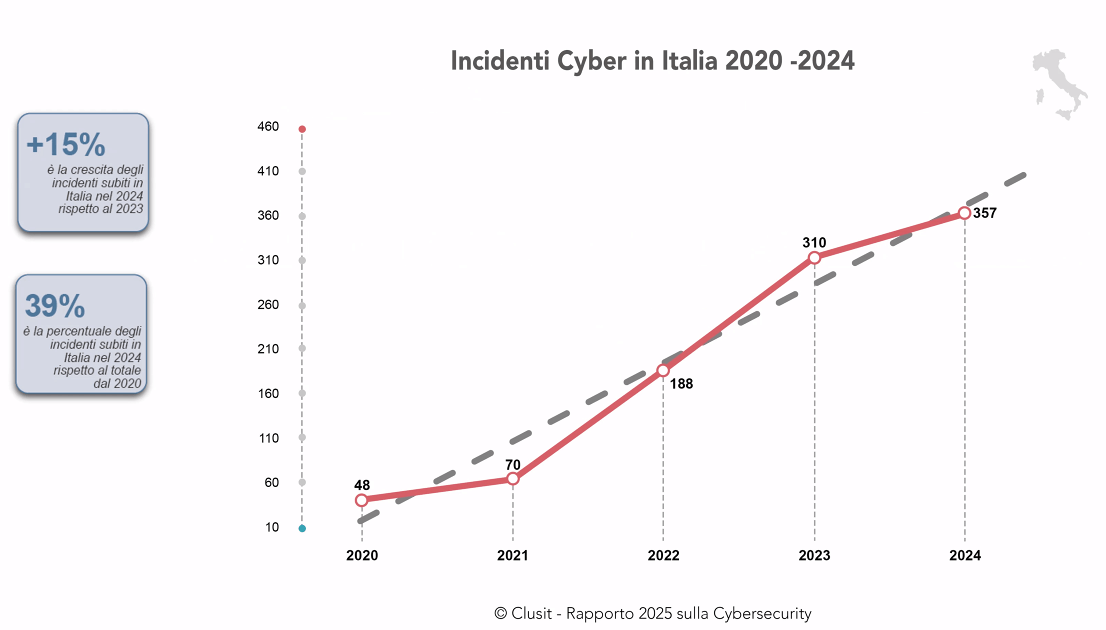
\includegraphics[width=1\linewidth]{images/intro/clusit-ita.png}
\end{figure}

In questo scenario, la Digital Forensics è diventata una competenza essenziale per qualsiasi organizzazione che voglia proteggere i propri asset digitali e rispondere efficacemente agli incidenti di sicurezza. Questa disciplina rappresenta oggi un pilastro fondamentale della cybersecurity aziendale, fornendo le capacità necessarie per rilevare attività malevole che i sistemi di sicurezza tradizionali potrebbero aver mancato, comprendere la portata e l'impatto di un incidente di sicurezza, contenere la minaccia e prevenire ulteriori danni, recuperare i sistemi compromessi e ripristinare le operazioni normali, e infine apprendere dall'incidente per migliorare le difese future.

\subsection{Il ruolo critico dell'analisi della memoria nei processi investigativi}

Tra le varie tecniche di Digital Forensics, l'analisi della memoria RAM occupa una posizione privilegiata. A differenza dell'analisi del disco, che esamina dati persistenti, l'analisi della memoria cattura lo stato "vivo" del sistema al momento dell'acquisizione. Questa capacità unica permette di osservare i processi in esecuzione, compresi quelli nascosti o offuscati dai rootkit che sfuggirebbero a un'analisi tradizionale. Simultaneamente, le connessioni di rete attive rivelano comunicazioni in corso con server di comando e controllo, mentre le chiavi crittografiche, normalmente protette, appaiono in chiaro durante il loro utilizzo. L'analisi della memoria espone inoltre gli artefatti di malware più sofisticati – dal codice iniettato agli hook di sistema, dalle modifiche al kernel alle credenziali temporaneamente decriptate – fornendo una visione completa dell'attività malevola che sarebbe altrimenti invisibile.

L'importanza dell'analisi della memoria è cresciuta esponenzialmente con l'evoluzione delle tecniche di attacco. I moderni malware sono progettati per operare esclusivamente in memoria (fileless malware), lasciando poche o nessuna traccia sul disco. Tecniche come process injection, reflective DLL injection e living-off-the-land rendono l'analisi della memoria non solo utile, ma spesso l'unico modo per rilevare e comprendere un attacco sofisticato.

\subsection{Sfide attuali}

L'analisi della memoria, nonostante la sua importanza critica, continua a incontrare ostacoli significativi che ne limitano la diffusione su larga scala. La complessità tecnica rappresenta la prima barriera: questa disciplina richiede non solo padronanza degli strumenti, ma una comprensione profonda delle strutture interne del sistema operativo, dei meccanismi di gestione della memoria e delle tecniche di anti-forensics adottate dai malware moderni. Tale curva di apprendimento scoraggia molti professionisti che, di fronte alla scelta, preferiscono concentrarsi su domini più consolidati come l'analisi di file system o di log di rete.

A questa complessità intrinseca si somma la sfida del volume dei dati. I sistemi moderni, dotati di decine o centinaia di gigabyte di RAM, producono dump di dimensioni proibitive per un'analisi manuale, richiedendo strumenti automatizzati e tecniche di filtraggio sofisticate per isolare gli artefatti significativi. La natura volatile della memoria aggiunge ulteriore pressione temporale: ogni secondo che passa dopo un incidente aumenta il rischio che evidenze cruciali vengano sovrascritte, trasformando l'acquisizione in una corsa contro il tempo che richiede procedure tanto rapide quanto affidabili.

Dal punto di vista strumentale, l'ecosistema delle soluzioni per la memory forensics rimane frammentato. Il framework open source Volatility rappresenta lo standard di fatto, ma richiede competenze da linea di comando e restituisce output che devono essere interpretati con grande esperienza. Le soluzioni commerciali alternative, pur offrendo interfacce più intuitive, spesso presentano costi elevati e funzionalità che non sempre giustificano l'investimento. La mancanza di automazione nelle operazioni critiche – dall'identificazione dei pattern sospetti alla correlazione tra artefatti, fino alla stesura dei report – trasforma attività che potrebbero essere standardizzate in processi manuali e time-consuming.

L'integrazione dei risultati dell'analisi della memoria con altre fonti di intelligence rappresenta un'ulteriore sfida. La correlazione con log applicativi, traffico di rete o feed di threat intelligence rimane un processo in larga parte artigianale e suscettibile di errori, compromettendo la visibilità complessiva dell'incidente e rallentando la risposta.

È proprio per rispondere a queste sfide che nascono piattaforme come VolWeb \cite{volweb2024}, concepite per democratizzare l'accesso alla memory forensics attraverso interfacce intuitive, automazioni intelligenti e capacità di correlazione avanzate, riducendo drasticamente la barriera d'ingresso e aumentando l'efficacia delle investigazioni.

\section{Obiettivi della Tesi}

Questo lavoro di tesi si propone di affrontare le sfide identificate attraverso l'espansione e il miglioramento di VolWeb, una piattaforma web-based per l'analisi forense della memoria. L'obiettivo principale consiste nell'integrazione di un sistema completo per la gestione e l'applicazione di regole YARA, strumento fondamentale per l'identificazione di pattern e malware nei dump di memoria. 

Questa integrazione, dettagliata nel Capitolo 5, mira a trasformare VolWeb in una piattaforma capace di gestire centralmente le regole YARA, applicarle efficacemente durante le analisi forensi e presentare i risultati in modo che faciliti l'interpretazione da parte degli analisti. Il sistema proposto permette non solo l'upload e la validazione delle regole, ma anche la loro organizzazione in rulesets logici, facilitando l'applicazione sistematica di intere categorie di pattern durante le investigazioni.

Il secondo obiettivo riguarda la validazione della piattaforma in contesti operativi reali, presentata nel Capitolo 6, con particolare riferimento alla preparazione per l'esercitazione NATO CCDCOE Locked Shields 2026. Questa validazione include stress test della piattaforma in condizioni di carico elevato, con analisi concorrenti di dump multipli, situazione tipica durante incident response su larga scala dove molteplici endpoint devono essere analizzati simultaneamente. La sperimentazione sul campo fornisce inoltre metriche concrete sull'efficacia delle espansioni implementate e feedback operativo per future ottimizzazioni.

Questi obiettivi non sono meramente tecnici, ma rispondono a un'esigenza concreta del mondo della cybersecurity: rendere l'analisi della memoria accessibile, efficiente e integrata nel workflow di incident response moderno. I capitoli che seguono tracciano il percorso completo dalla teoria alla pratica: il Capitolo 2 fornisce le basi teoriche del DFIR e della memory forensics, il Capitolo 3 analizza VolWeb nella sua versione originale, il Capitolo 4 presenta l'esperienza di Locked Shields che ha motivato le espansioni, il Capitolo 5 dettaglia l'implementazione delle nuove funzionalità, il Capitolo 6 ne valida l'efficacia sul campo, e infine le conclusioni sintetizzano i risultati raggiunti e delineano le prospettive future.
\chapter{Background e Stato dell'Arte}

L'evoluzione del panorama delle minacce informatiche ha reso indispensabile lo sviluppo di tecniche e strumenti sempre più sofisticati per l'analisi forense digitale. Questo capitolo fornisce le basi teoriche necessarie per comprendere il contesto in cui si inserisce il presente lavoro, esplorando i concetti fondamentali del Digital Forensics and Incident Response (DFIR), con particolare attenzione all'analisi della memoria volatile. Verranno inoltre esaminati i principali framework esistenti, con focus su Volatility e YARA, evidenziando le limitazioni che motivano le espansioni proposte in questa tesi.

\section{Digital Forensics e Incident Response (DFIR)}

\subsection{Definizione e principi fondamentali}

Il Digital Forensics and Incident Response (DFIR) rappresenta la convergenza di due discipline complementari che, insieme, formano il nucleo delle capacità di risposta alle minacce cyber moderne. Il termine DFIR è stato coniato per riflettere la natura interconnessa di queste attività nel contesto operativo reale.

La Digital Forensics é definita come \textit{l'applicazione di tecniche scientifiche per l'identificazione, raccolta, analisi e presentazione di evidenze digitali in modo che siano ammissibili in tribunale}" \cite{palmer2001} e si fonda su quattro principi scientifici fondamentali che ne garantiscono il rigore metodologico \cite{kent2006}. La preservazione dell'evidenza assicura che i dati non vengano alterati durante l'acquisizione e l'analisi, mentre la chain of custody documenta ogni passaggio per mantenere l'ammissibilità legale delle prove. A questi si aggiungono la ripetibilità delle analisi, che devono produrre risultati consistenti, e la documentazione completa di ogni azione intrapresa, elementi che insieme formano il framework metodologico codificato negli standard internazionali come ISO/IEC 27037:2012 \cite{iso27037}.

Questi principi sono ulteriormente rafforzati dalle linee guida SWGDE \cite{swgde2022} che stabiliscono best practices specifiche per la preservazione di evidenze volatili come pagine web, social media e comunicazioni cloud-based, riflettendo l'evoluzione delle fonti di evidenza nell'era digitale moderna.

L'Incident Response si concentra invece sulla gestione operativa degli incidenti di sicurezza con l'obiettivo di minimizzare l'impatto e ripristinare le operazioni normali nel minor tempo possibile. Il SANS Institute la definisce come "un approccio organizzato per affrontare e gestire le conseguenze di una violazione della sicurezza o di un attacco informatico" \cite{sans2023}.

La fusione di queste discipline nel DFIR riconosce che, nel mondo reale, l'analisi forense e la risposta agli incidenti sono attività inseparabili. Durante un incidente attivo, i responder devono bilanciare molteplici esigenze contrastanti: contenere la minaccia mentre preservano le evidenze, analizzare i sistemi compromessi senza interrompere le operazioni critiche, e trovare il giusto equilibrio tra la necessità di un'indagine approfondita e l'urgenza del ripristino operativo.

\subsection{Il processo DFIR}

Il processo DFIR segue un approccio metodologico articolato in sei fasi distinte, come definito dal framework NIST SP 800-61 \cite{cichonski2012}. Sebbene questa struttura fornisca un modello logico di riferimento, nella pratica operativa le fasi si sovrappongono frequentemente e richiedono un approccio iterativo.

\begin{figure}[H]
    \centering
    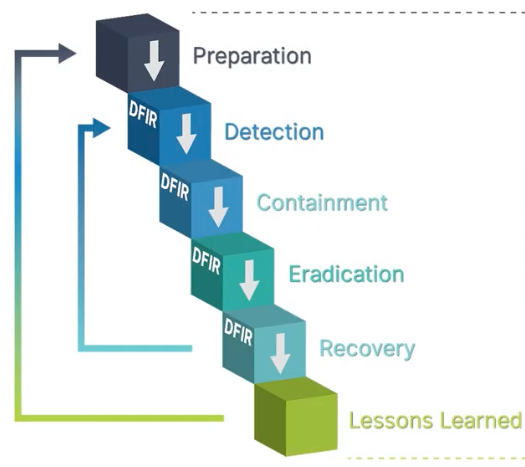
\includegraphics[width=0.6\linewidth]{images/stato-arte/digital-forensics-incident-response-plan-flow.png}
\end{figure}

La preparazione rappresenta il fondamento dell'intero processo, determinando la differenza tra una risposta efficace e una gestione caotica. Questa fase richiede lo sviluppo preventivo di playbook e procedure operative standard, supportati da un'infrastruttura tecnologica adeguata e training continuo del personale. L'identificazione inizia con l'analisi degli alert provenienti dai sistemi di sicurezza, seguita da un processo di triage che distingue i falsi positivi dalle minacce concrete. Il contenimento diventa poi prioritario per limitare la propagazione del danno attraverso azioni immediate di isolamento e misure sostenibili a lungo termine, sempre preservando le evidenze forensi.

L'eradicazione richiede un approccio sistematico che va oltre la rimozione degli artefatti visibili, identificando tutti i componenti malevoli, incluse backdoor e meccanismi di persistenza nascosti. Il recupero rappresenta una fase delicata dove la ricostruzione deve partire da backup verificati, accompagnata da monitoraggio intensificato. Infine, la fase di lessons learned trasforma ogni incidente in un'opportunità di miglioramento attraverso documentazione dettagliata e analisi critica.

Il DFIR è ormai essenziale nella cybersecurity moderna sia per fronteggiare minacce avanzate come APT e ransomware, sia per rispondere a requisiti normativi stringenti come il GDPR \cite{gdpr2016} che impone notifica entro 72 ore, la direttiva NIS2 \cite{nis2_2022} per operatori essenziali, e il DORA \cite{dora2022} per il settore finanziario. Con il tempo medio di permanenza degli attaccanti sceso a 16 giorni \cite{mandiant2023}, la capacità di risposta rapida ed efficace diventa critica.

\section{Memory Forensics}

\subsection{La memoria volatile come fonte di evidenze}

La memoria volatile, principalmente la RAM, rappresenta lo stato "vivo" di un sistema informatico catturando informazioni effimere ma fondamentali che rivelano con precisione cosa stava accadendo al momento dell'acquisizione \cite{ligh2014}. A differenza dello storage persistente, la memoria offre una finestra unica sui processi in esecuzione, le connessioni di rete attive, e i dati temporaneamente decifrati.

L'architettura della memoria segue una gerarchia complessa che parte dai registri CPU ultra-veloci ma minuscoli, attraversa le cache L1-L3 progressivamente più capienti, e culmina nella RAM principale che costituisce l'area di lavoro del sistema. Questa contiene lo spazio kernel con le strutture critiche del sistema operativo, lo spazio utente dove risiedono processi e applicazioni, la pool memory per allocazioni dinamiche, e la page cache con i dati dei file recenti.

La gestione della memoria virtuale aggiunge complessità ma anche opportunità investigative. Ogni processo opera in uno spazio di indirizzamento isolato, con pagine virtuali mappate dinamicamente su frame fisici attraverso page tables e translation lookaside buffers. Per l'analista forense, ricostruire questi mapping è essenziale per interpretare correttamente il contenuto della memoria \cite{case2017}.

\subsection{Artefatti recuperabili e vantaggi dell'analisi}

La memoria volatile conserva artefatti unici non reperibili altrove. I processi e thread rivelano l'intera lista dei processi, inclusi quelli nascosti da rootkit, con argomenti command line, variabili d'ambiente, handle aperti, stack e heap contenenti tracce dell'esecuzione. Le informazioni di rete mostrano connessioni TCP/UDP attive, socket in ascolto che potrebbero nascondere backdoor, cache DNS e buffer di pacchetti.

Particolarmente critici sono gli artefatti di sicurezza: token di autenticazione e chiavi crittografiche temporaneamente in chiaro, certificati SSL/TLS, ticket Kerberos, hash NTLM e password di applicazioni. Le evidenze di malware includono codice iniettato in processi legittimi, API hooks, driver kernel malevoli, payload cifrati decriptati solo a runtime, e comunicazioni C\&C. Le tracce di attività utente comprendono clipboard, titoli di finestre, cronologia comandi, documenti in editing e chat in chiaro.

L'analisi della memoria offre vantaggi unici rispetto all'analisi del disco. Garantisce visibilità su minacce fileless e tecniche living-off-the-land che non lasciano tracce su disco. Permette l'accesso a dati normalmente cifrati, osservabili in chiaro durante l'esecuzione. Fornisce una visione runtime completa con processi, connessioni e allocazioni dinamiche, con una timeline difficilmente falsificabile. Inoltre, bypassa molte contromisure anti-forensi poiché modifiche ai file o cancellazioni secure non influenzano le strutture in RAM.

\section{Framework e Strumenti per l'Analisi della Memoria}

\subsection{Volatility Framework}

Volatility \cite{volatility2024} rappresenta lo standard de facto per l'analisi forense della memoria dal suo rilascio nel 2007. Creato inizialmente da Aaron Walters per democratizzare l'accesso a tecniche precedentemente riservate a poche agenzie, il framework si è evoluto attraverso tre versioni maggiori. Volatility 2.0 (2011) introdusse l'architettura plugin-based che ne permise l'espansione da parte della community. Volatility 3 (2019) rappresentò una riscrittura completa in Python 3, risolvendo limitazioni architetturali accumulate e migliorando significativamente le performance.

L'architettura di Volatility 3 si basa su componenti modulari elegantemente integrati. Il Framework Core orchestra configurazione ed esecuzione, mentre le Symbol Tables permettono di interpretare le strutture dati specifiche di ogni versione di sistema operativo. Gli Address Spaces forniscono astrazione per diversi formati di dump, i Plugins implementano la logica di estrazione degli artefatti, e i Renderers gestiscono l'output in formati multipli.

Il framework offre oltre 100 plugin che coprono ogni aspetto dell'analisi. Per l'analisi dei processi, \texttt{pstree} visualizza relazioni gerarchiche evidenziando anomalie parent-child spesso indicative di injection, mentre \texttt{psscan} esegue scansioni euristiche per scoprire processi nascosti da rootkit. L'estrazione delle command line con \texttt{cmdline} rivela gli obiettivi degli attaccanti, e l'analisi di DLL e handle fornisce insight sulle risorse manipolate.

Per l'analisi di rete, \texttt{netscan} (ottimizzato per Windows Vista+) fornisce una visione comprensiva delle connessioni, evoluzione dei precedenti plugin per sistemi legacy. La detection di malware si avvale di \texttt{malfind} che implementa euristiche sofisticate per identificare code injection cercando pagine eseguibili non mappate a file - combinazione altamente sospetta. Plugin complementari come \texttt{hollowfind} specializzano la ricerca verso process hollowing, mentre l'analisi dei callback kernel può rivelare rootkit a livello kernel.

\subsection{YARA}

YARA \cite{yara2024}, creato da Victor M. Alvarez presso VirusTotal nel 2008, è diventato lo standard per pattern matching e classificazione di malware. Il suo successo deriva dalla capacità di descrivere famiglie di malware attraverso regole basate su caratteristiche testuali o binarie, applicabili a file, processi o dump di memoria.

La sintassi YARA bilancia espressività e semplicità. Una regola tipica contiene tre sezioni: \textbf{meta} con metadati descrittivi, \textbf{strings} che definisce i pattern da cercare (stringhe, hex, regex), e \textbf{condition} che specifica la logica booleana per il matching. 

\begin{minted}[
    breaklines,
    frame=lines,
    framesep=2mm,
    baselinestretch=1.2,
    fontsize=\small,
    linenos
]{c}
rule ExampleRule {
    meta:
        author = "Security Researcher"
        description = "Detects Example Malware"
        date = "2024-01-01" 
    strings:
        $text_string = "malicious_function"
        $hex_string = { 6A 40 68 00 30 00 00 6A 14 8D }
        $regex = /\w+\.exe/
    condition:
        any of them
}
\end{minted}

La flessibilità delle condizioni permette logiche detection estremamente sofisticate utilizzando operatori logici, contatori, offset e funzioni built-in. Le condizioni possono essere semplici ("any of them") o complesse, combinando multipli criteri per ridurre i falsi positivi e aumentare l'accuratezza del rilevamento.

Quando applicato alla memoria, YARA trasforma le capacità investigative. Eccelle nell'identificare malware che esistono solo runtime - shellcode iniettato in processi legittimi, DLL reflective che non toccano disco, payload che si materializzano solo post-exploitation. Durante il threat hunting, YARA cerca stringhe uniche di famiglie malware specifiche, pattern di comunicazione C2, o artefatti di tool post-exploitation come Cobalt Strike.

La vera potenza emerge nel rilevamento di tecniche di evasione. YARA può identificare pattern lasciati da process hollowing dove processi legittimi vengono svuotati e riempiti con codice malevolo, riconoscere API hooks sospetti, o pattern di allocazione memoria che tradiscono injection avanzate. Ogni tecnica di evasione, per quanto sofisticata, lascia inevitabilmente una firma che YARA può essere addestrata a riconoscere.

Volatility integra nativamente YARA attraverso il plugin \texttt{yarascan}, che non si limita a segnalare match ma fornisce ricco contesto forense: offset di memoria per correlazioni, processo proprietario per attribuzione, permessi della pagina (RWX spesso indica injection), e dump del contenuto circostante per analisi manuale approfondita.

\subsection{Limitazioni degli approcci attuali}

Nonostante la maturità degli strumenti disponibili, l'adozione della memory forensics rimane limitata da barriere sistemiche che ne impediscono il pieno potenziale.

La complessità tecnica costituisce l'ostacolo principale. L'analisi efficace richiede non solo competenza sui tool ma comprensione profonda di architetture OS, gestione memoria, e tecniche anti-forensics. Interpretare i risultati necessita esperienza per distinguere comportamenti normali da anomalie in contesti diversi. La necessità di scripting per automazione esclude personale non programmatore, creando un collo di bottiglia nelle capacità investigative delle organizzazioni.

L'interfaccia command-line di Volatility, per quanto potente per utenti esperti, rallenta significativamente il processo di triage iniziale quando ogni minuto conta. L'output testuale non strutturato richiede post-processing manuale intensivo per identificare informazioni rilevanti, mentre l'integrazione limitata con YARA impedisce ricerche complesse basate su pattern comportamentali. L'assenza di funzionalità collaborative native rappresenta un ulteriore ostacolo in contesti dove il lavoro di team è essenziale.

Gli strumenti commerciali come Magnet AXIOM e Mandiant Redline, pur offrendo interfacce più intuitive, presentano limitazioni critiche in contesti competitivi. I modelli di licensing restrittivi limitano l'accesso simultaneo necessario per team numerosi, mentre le capacità di customizzazione limitate impediscono l'implementazione rapida di nuove tecniche analitiche richieste da scenari in evoluzione.

L'assenza di standard condivisi e l'incompatibilità tra strumenti creano inefficienze sistemiche che si amplificano sotto pressione temporale. La necessità di utilizzare tool multipli per coprire l'intero spettro di requisiti introduce overhead significativo nel trasferimento di dati e contesto. I problemi di scalabilità emergono in scenari enterprise dove incidenti coinvolgono centinaia di endpoint. L'analisi sequenziale di dump multipli diventa proibitiva senza parallelizzazione nativa.

L'integrazione limitata con l'ecosistema di sicurezza riduce il valore operativo. Threat intelligence feeds non si integrano nativamente, la correlazione con logs e network traffic è manuale, export verso piattaforme avanzate richiede trasformazioni complesse, e API limitate impediscono automazione enterprise-grade.

Le limitazioni identificate negli approcci tradizionali hanno creato lo spazio per soluzioni innovative come VolWeb \cite{volweb2024}, che si propone di colmare il gap tra la potenza analitica di Volatility e l'accessibilità richiesta dai moderni team di sicurezza. Il prossimo capitolo esamina in dettaglio come VolWeb affronta queste sfide attraverso la sua architettura web-based e l'approccio user-centric.
\chapter{VolWeb: La Piattaforma Web per Volatility}

L'evoluzione degli strumenti di digital forensics ha sempre seguito un percorso che bilancia potenza analitica e accessibilità. In questo contesto, VolWeb emerge come una soluzione innovativa che affronta una delle sfide più significative nell'adozione della memory forensics: la complessità d'uso degli strumenti esistenti. Sviluppato come progetto open source, VolWeb si propone di rendere le capacità avanzate di Volatility 3 accessibili attraverso un'interfaccia web moderna, eliminando molte delle barriere che tradizionalmente hanno limitato l'adozione di queste tecniche investigative.

Il presente capitolo analizza in dettaglio gli aspetti tecnici dell'implementazione, le scelte architetturali e le capacità forensi offerte dalla piattaforma nella sua versione originale.

\section{Il contesto e gli obiettivi di VolWeb}

VolWeb \cite{volweb2024} nasce dalla constatazione di un paradosso nel campo della memory forensics: mentre Volatility si è affermato come lo standard per l'analisi della memoria, le limitazioni discusse nel capitolo precedente (Sezione 2.3.3) ne hanno di fatto limitato l'adozione a una ristretta cerchia di specialisti con competenze tecniche avanzate. Questa situazione crea un collo di bottiglia operativo in molte organizzazioni, dove la capacità di analizzare rapidamente dump di memoria può fare la differenza tra contenere un incidente o subirne le conseguenze complete.

Il progetto, avviato nel 2023, si inserisce in un momento storico particolare per la cybersecurity. L'aumento esponenziale degli attacchi ransomware, la sofisticazione crescente delle Advanced Persistent Threats e l'adozione massiva del lavoro remoto hanno moltiplicato la superficie di attacco delle organizzazioni. In questo scenario, la capacità di condurre analisi forensi rapide ed efficaci diventa non più un lusso per pochi specialisti, ma una necessità operativa diffusa.

In risposta a queste sfide, VolWeb persegue tre obiettivi fondamentali strettamente interconnessi. Il primo è la democratizzazione dell'accesso alle capacità di memory forensics attraverso un'interfaccia che nasconda la complessità di Volatility senza sacrificarne la potenza. Questo obiettivo si concretizza nella riduzione del tempo necessario per ottenere risultati actionable da ore a minuti, permettendo anche ad analisti con esperienza limitata di condurre investigazioni efficaci. 

Il secondo obiettivo riguarda la standardizzazione dei workflow investigativi. Mentre l'uso diretto di Volatility lascia ampia libertà nell'approccio all'analisi, questa flessibilità può tradursi in inconsistenza e inefficienza, specialmente in team con membri di diversa esperienza. VolWeb introduce quindi un framework strutturato che guida l'analista attraverso le fasi dell'investigazione, garantendo completezza e riproducibilità. 

Il terzo pilastro è rappresentato dalla collaborazione, essenziale nelle investigazioni moderne che raramente coinvolgono un singolo analista ma richiedono il coordinamento di team distribuiti geograficamente e temporalmente. VolWeb fornisce un ambiente condiviso dove più analisti possono lavorare sugli stessi casi, condividere osservazioni e costruire collettivamente la comprensione di un incidente.


\section{Principi architetturali}

L'architettura di VolWeb riflette una filosofia di design che privilegia modularità, estensibilità e manutenibilità. La scelta di un'architettura web-based deriva da considerazioni pratiche sull'uso reale dello strumento in contesti operativi. Gli analisti forensi operano spesso in condizioni di emergenza, da postazioni diverse e con risorse hardware variabili. Un'applicazione web elimina le frizioni legate all'installazione e configurazione di software complesso, permettendo un accesso immediato alle funzionalità di analisi.

La separazione tra frontend e backend attraverso API REST \cite{restapi} rappresenta una scelta architettonica fondamentale che va oltre la semplice modularizzazione del codice. Questa separazione permette l'evoluzione indipendente dei componenti, facilitando sia lo sviluppo che la manutenzione. Inoltre, esporre le funzionalità attraverso API standardizzate apre la possibilità di integrazioni con altri strumenti dell'ecosistema di sicurezza, trasformando VolWeb da applicazione standalone a componente di pipeline di analisi più ampie.

\subsection{Stack tecnologico}

\begin{figure}[H]
    \centering
    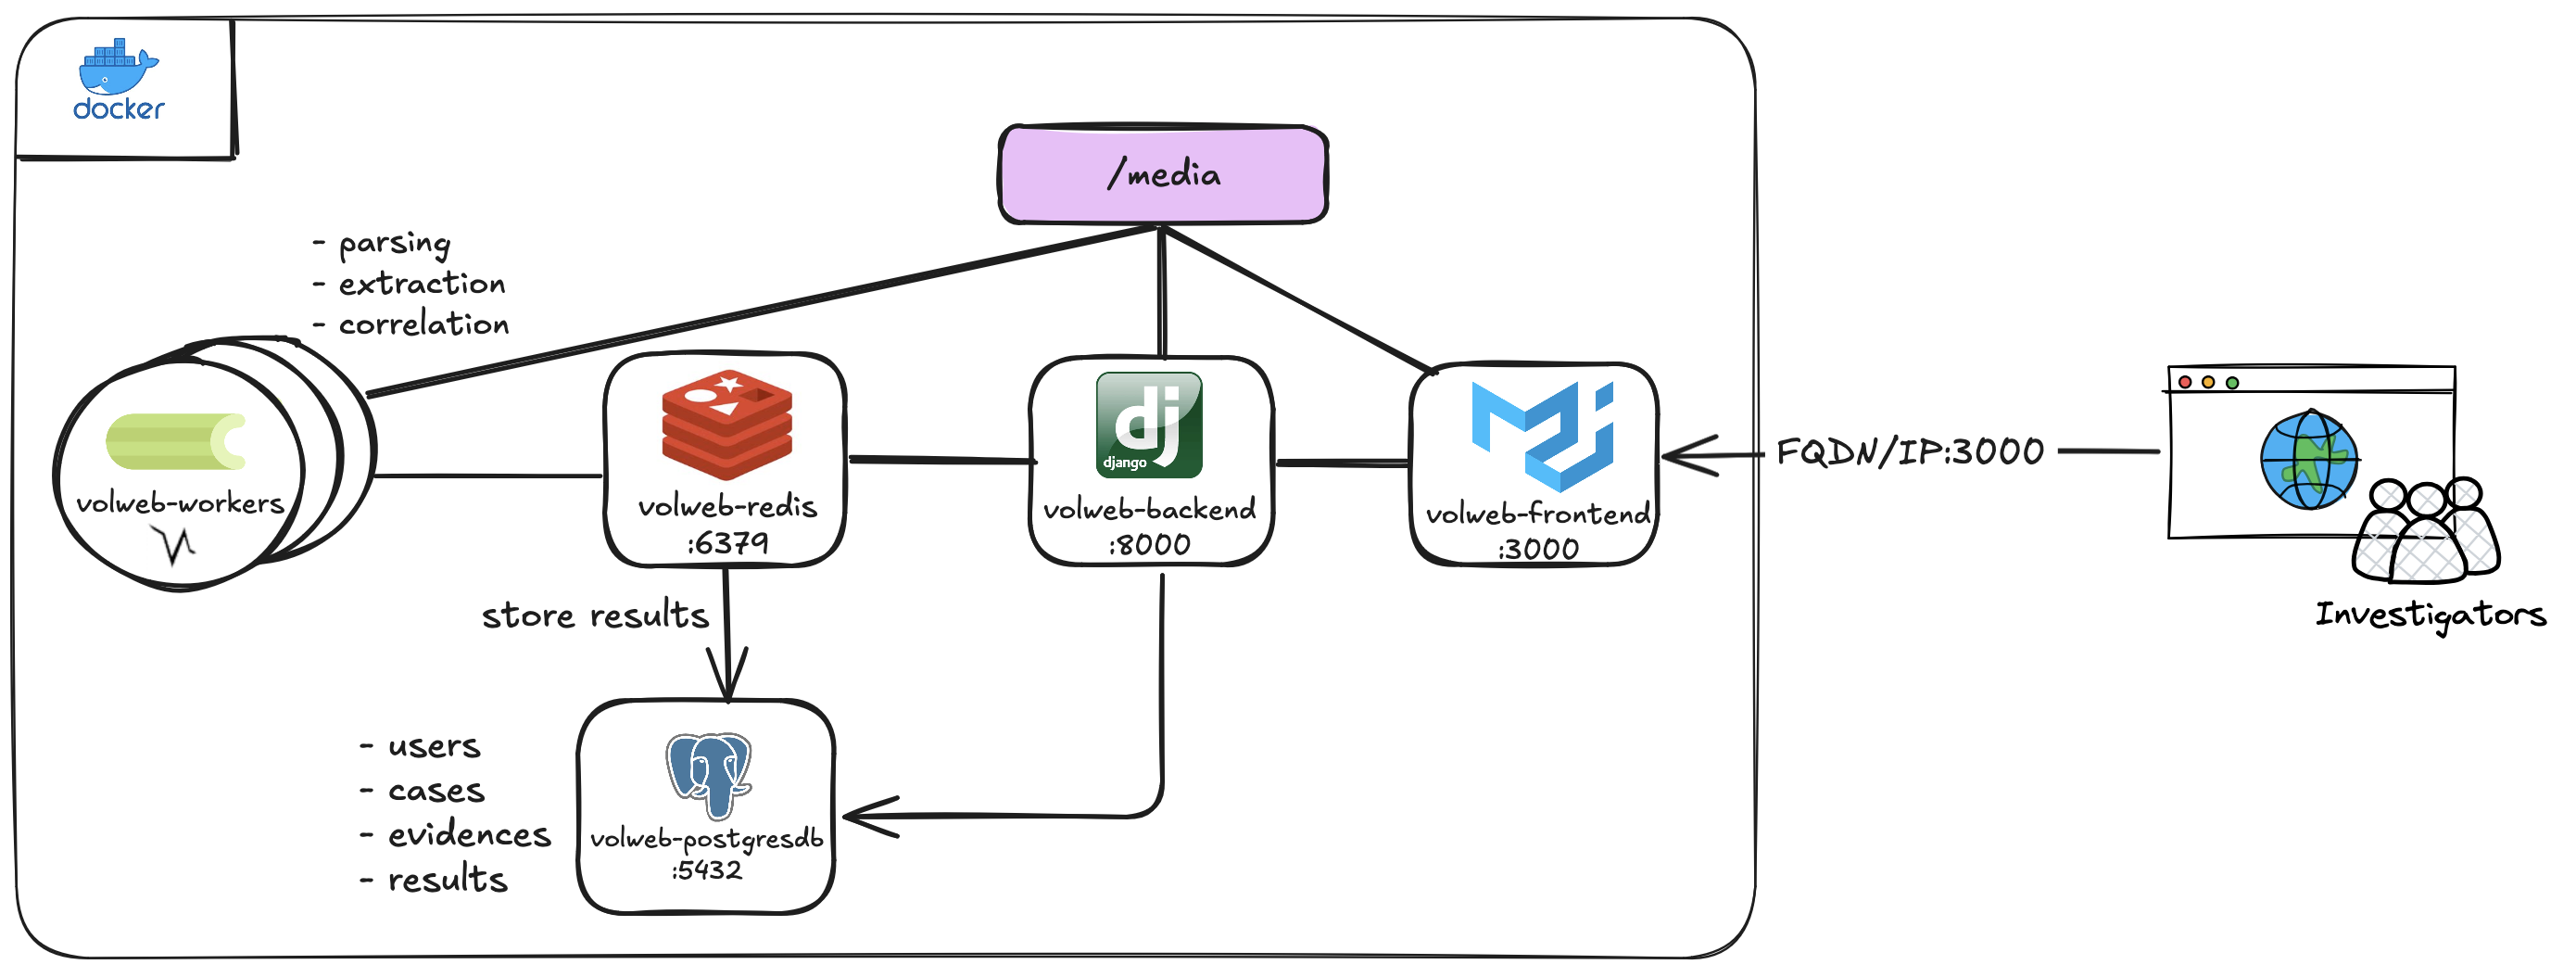
\includegraphics[width=1\linewidth]{images/volweb-original/volweb-arch.png}
\end{figure}

La selezione delle tecnologie utilizzate in VolWeb riflette un bilanciamento tra maturità, performance e facilità di sviluppo. Il backend, costruito su \textbf{Django 4.2} e \textbf{Django REST Framework}, sfrutta un ecosistema consolidato che offre soluzioni robuste per problematiche comuni come autenticazione, gestione delle sessioni e validazione dei dati. La scelta di Django non è casuale: il framework Python si integra naturalmente con Volatility 3, permettendo un'interazione diretta senza layer di traduzione aggiuntivi.

Il frontend utilizza \textbf{React 18.2.0} con \textbf{Material-UI 5.14} per l'interfaccia utente. Questa combinazione fornisce un'esperienza utente moderna e reattiva, fondamentale per mantenere l'efficienza operativa durante investigazioni che possono protrarsi per ore. La scelta di Material-UI come design system garantisce consistenza visiva e accessibilità, aspetti spesso trascurati nei tool forensi ma cruciali per ridurre il carico cognitivo dell'analista durante sessioni di analisi intensive.

Per la gestione dei task asincroni, VolWeb si affida a \textbf{Celery 5.3} con \textbf{Redis} come message broker. Questa architettura permette di gestire operazioni computazionalmente intensive come l'analisi di dump di memoria di grandi dimensioni senza bloccare l'interfaccia utente. La scalabilità orizzontale offerta da Celery consente inoltre di distribuire il carico di lavoro su molteplici macchine, aspetto critico quando si devono analizzare contemporaneamente dump provenienti da decine di endpoint compromessi.

La persistenza dei dati è affidata a \textbf{PostgreSQL}, scelto per la sua affidabilità e le capacità avanzate di gestione di dati JSON, particolarmente utili per memorizzare i risultati strutturati ma eterogenei prodotti dai vari plugin di Volatility. L'uso di SQLite come alternativa per deployment di sviluppo o di piccola scala dimostra l'attenzione alla flessibilità di deployment, permettendo agli sviluppatori di avere un ambiente funzionale senza la complessità di configurare un database server completo.

\subsection{Integrazione con Volatility 3}

Il cuore tecnico di VolWeb risiede nell'integrazione con Volatility 3, realizzata attraverso un layer di astrazione che gestisce la complessità dell'interazione con il framework. Questa integrazione non si limita a un semplice wrapper delle funzionalità command-line, ma implementa una gestione sofisticata del ciclo di vita dell'analisi.

Il modulo definito in 'backend/volatility\_engine.py' implementa un'interfaccia Python nativa con Volatility 3. Questo approccio elimina l'overhead dell'invocazione di processi esterni e permette un controllo granulare sull'esecuzione dei plugin. La gestione della configurazione di Volatility, tradizionalmente complessa e error-prone, viene automatizzata attraverso la costruzione dinamica del contesto di esecuzione basata sui metadati del dump analizzato.

Un aspetto particolarmente innovativo dell'integrazione riguarda la gestione dei simboli. Volatility richiede symbol tables specifiche per ogni versione di sistema operativo per interpretare correttamente le strutture dati in memoria. VolWeb automatizza il download e la gestione di questi simboli, eliminando uno dei principali ostacoli tecnici nell'uso di Volatility. Il sistema mantiene una cache locale dei simboli più comuni e scarica automaticamente quelli mancanti quando necessario. Inoltre, permette anche di caricare manualmente i file dei simboli direttamente dal file system, offrendo all'utente un controllo completo in caso di configurazioni particolari o ambienti offline.

La gestione degli errori rappresenta un altro aspetto critico dell'integrazione. I plugin di Volatility possono fallire per molteplici ragioni, dalla corruzione del dump all'incompatibilità con la versione del sistema operativo. VolWeb implementa una strategia di error handling che distingue tra errori fatali e warning, permettendo all'analisi di procedere anche quando singoli plugin falliscono, mentre registra dettagliatamente le cause del fallimento per troubleshooting successivo.

\subsection{Requisiti di sistema e installazione}

Prima di procedere con l'installazione di VolWeb, è necessario verificare che l'ambiente soddisfi i requisiti minimi. Il sistema richiede \textbf{Python 3.8 o superiore}, fondamentale per la compatibilità con Volatility 3 e le librerie moderne utilizzate. È inoltre necessario avere Git installato per clonare il repository e Docker con Docker Compose per il deployment containerizzato, che rappresenta il metodo di installazione raccomandato.

Dal punto di vista hardware, sebbene VolWeb possa funzionare su sistemi modesti per analisi di piccola scala, per un utilizzo produttivo si raccomandano almeno 8 GB di RAM e storage sufficiente per i dump di memoria, che possono facilmente raggiungere decine di gigabyte per sistema analizzato. La disponibilità di CPU multi-core è fortemente raccomandata per sfruttare appieno le capacità di elaborazione parallela offerte da Celery.

L'installazione di VolWeb è stata progettata per essere il più semplice possibile, riconoscendo che la complessità di setup è spesso una barriera all'adozione. Il processo standard prevede prima di tutto la clonazione del repository:

\begin{minted}[bgcolor=gray!10, fontsize=\small]{bash}
git clone https://github.com/k1nd0ne/VolWeb.git
cd VolWeb
\end{minted}

Successivamente, l'ambiente può essere avviato utilizzando Docker Compose, che gestisce automaticamente tutte le dipendenze e configurazioni:

\begin{minted}[bgcolor=gray!10, fontsize=\small]{bash}
docker-compose up -d
\end{minted}

La containerizzazione offre vantaggi significativi per la riproducibilità e la portabilità, garantendo che gli stessi container possano essere deployati in ambiente di sviluppo, test e produzione con comportamento consistente.

\section{Workflow Operativo e Gestione}

\subsection{Gestione dei casi}

Il workflow operativo di VolWeb inizia con la creazione di un caso, che rappresenta il contenitore logico per un'investigazione. Ogni caso può aggregare molteplici evidenze, permettendo l'analisi correlata di dump provenienti da sistemi diversi coinvolti nello stesso incidente. La gestione dei casi segue best practice forensi, mantenendo metadati completi su chi ha creato il caso, quando è stato modificato e quale sia il suo stato corrente.

\begin{figure}[H]
    \centering
    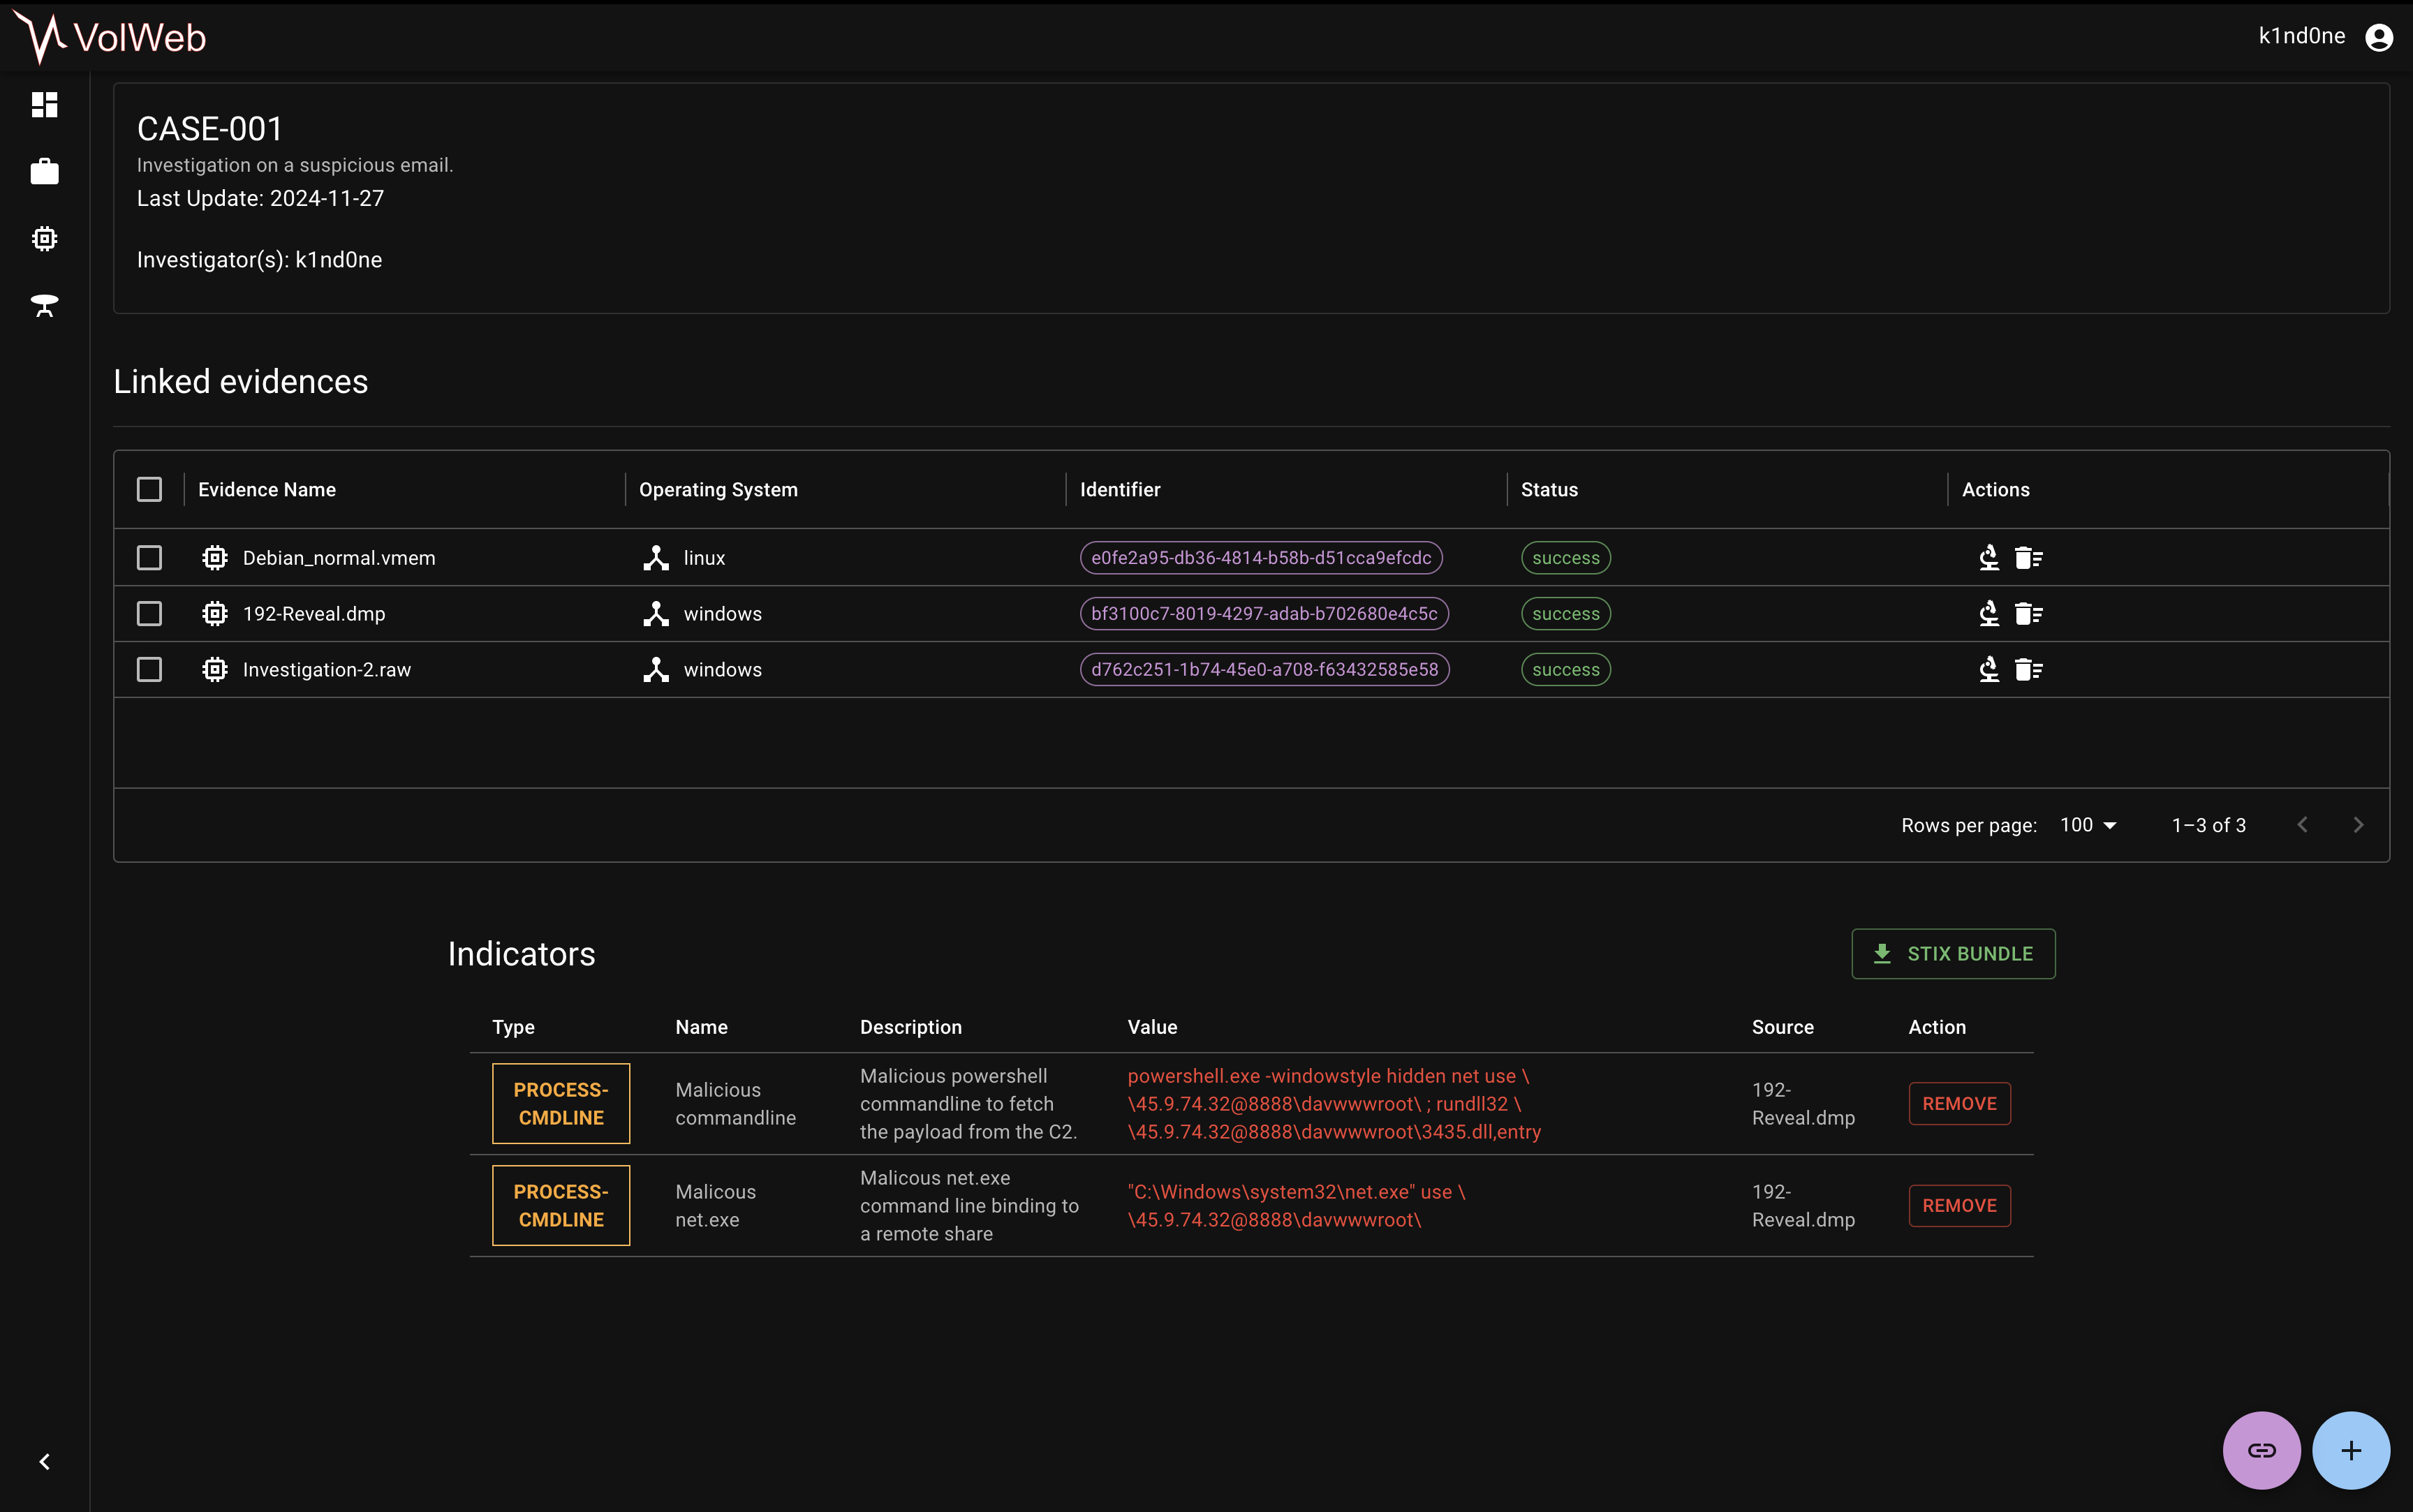
\includegraphics[width=1\linewidth]{images/volweb-original/volweb-case-management.png}
\end{figure}

L'interfaccia di gestione presenta una dashboard che fornisce una vista immediata dello stato delle investigazioni. Ogni caso è rappresentato da una card che mostra informazioni essenziali: nome, descrizione, numero di evidenze associate, stato dell'analisi e ultima modifica. Questa presentazione visiva permette agli analisti di prioritizzare rapidamente il proprio lavoro e identificare casi che richiedono attenzione immediata.

\subsection{Upload e Gestione dei Dump di Memoria}

Una volta creato un caso, il passo successivo è l'upload dei dump di memoria da analizzare. VolWeb gestisce questo processo critico con particolare attenzione all'integrità dei dati e all'esperienza utente. L'interfaccia di upload supporta drag-and-drop, permettendo agli utenti di trascinare file direttamente dal file manager del sistema operativo.

\begin{figure}[H]
    \centering
    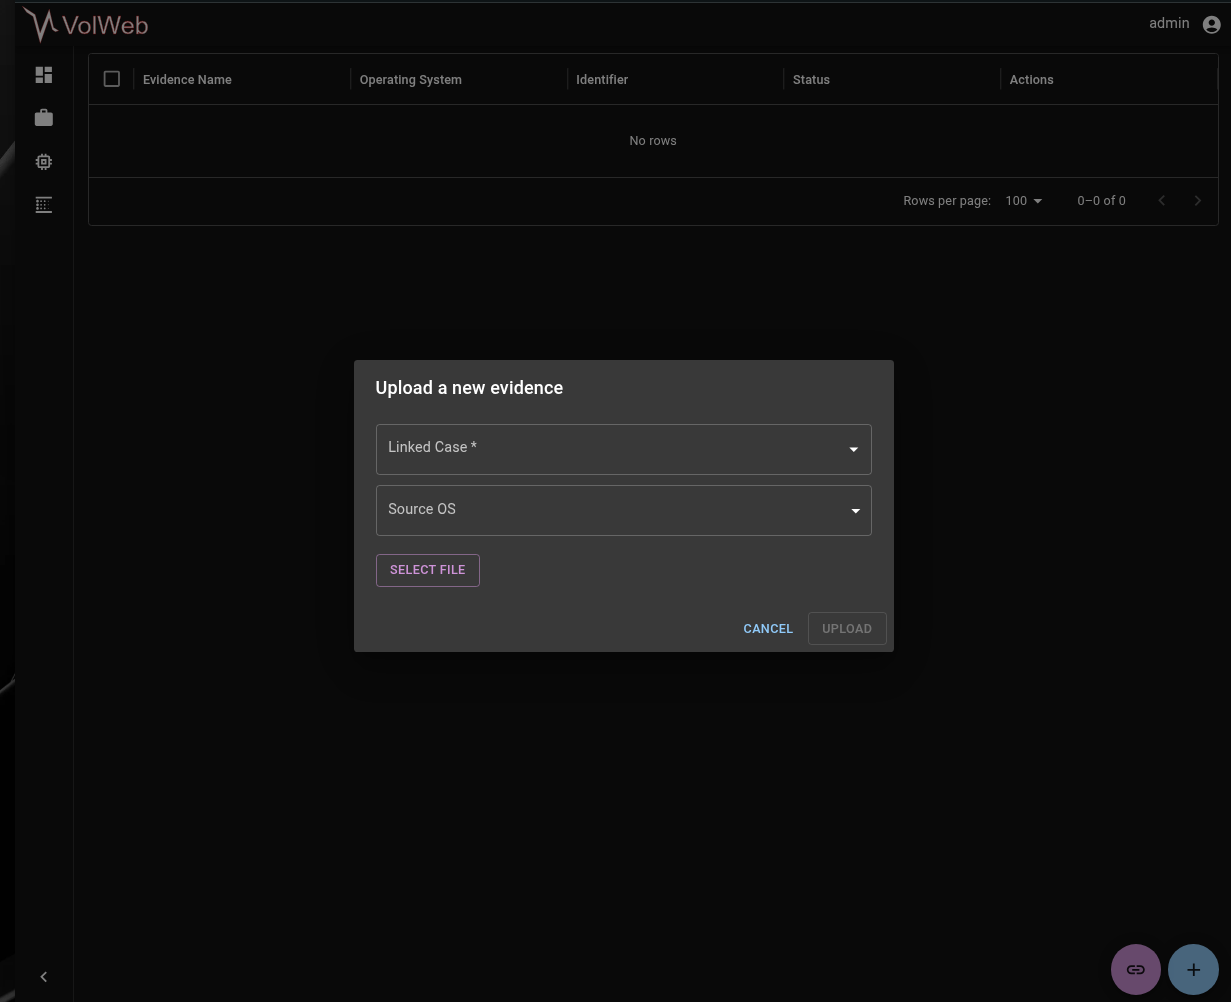
\includegraphics[width=0.9\linewidth]{images/volweb-original/volweb-upload-interface.png}
\end{figure}

La gestione di file di grandi dimensioni rappresenta una sfida tecnica significativa in un'applicazione web. I dump di memoria possono facilmente superare i 10 GB, dimensioni che mettono alla prova sia l'infrastruttura di rete che i meccanismi standard di upload HTTP. VolWeb affronta questa sfida attraverso un sistema sofisticato di gestione che combina upload chunked, validazione dell'integrità e rilevamento automatico del profilo.

Per file di grandi dimensioni, comune scenario con dump di memoria che possono superare i 16GB, VolWeb implementa un sistema di upload chunked. Questo approccio divide il file in blocchi più piccoli che vengono trasmessi sequenzialmente, con la possibilità di riprendere l'upload in caso di interruzione della connessione. Il backend gestisce l'assemblaggio dei chunk e la validazione dell'integrità attraverso hash crittografici, mantenendo metadati dettagliati su ogni file inclusi hash multipli per la verifica dell'integrità e timestamp per la chain of custody.

Uno degli aspetti più innovativi di VolWeb è il sistema di rilevamento automatico del profilo del sistema operativo. Questo processo, tradizionalmente manuale e soggetto a errori, viene automatizzato attraverso l'analisi delle strutture dati presenti nel dump. Il sistema esamina prima signature ad alta confidenza che permettono l'identificazione immediata. Se queste non producono risultati, procede con euristiche più complesse che analizzano pattern di strutture dati. Come fallback finale, l'utente può specificare manualmente il profilo, ma nella pratica questo è raramente necessario.

\subsection{Analisi automatica}

Dopo il completamento dell'upload, VolWeb avvia automaticamente una serie di analisi predefinite progettate per fornire una panoramica immediata del sistema analizzato. Questa suite di plugin include l'enumerazione dei processi attraverso \textbf{pslist}, l'analisi delle connessioni di rete con \textbf{netscan}, l'estrazione delle command line tramite \textbf{cmdline}, la lista delle DLL caricate utilizzando \textbf{dlllist} e l'identificazione degli handle aperti con \textbf{handles}.

La selezione di questi plugin non è casuale ma deriva dall'esperienza operativa che identifica queste informazioni come il minimo dataset necessario per una comprensione iniziale dello stato del sistema. L'esecuzione automatica elimina la necessità per l'analista di ricordare quali plugin eseguire per primi, standardizzando l'approccio investigativo.

Durante l'analisi, VolWeb fornisce feedback dettagliato attraverso WebSocket, mostrando quale plugin è in esecuzione, la percentuale di completamento e eventuali warning o errori. Questo feedback real-time è cruciale per mantenere la fiducia dell'utente durante operazioni che possono richiedere tempo significativo.

\section{Interfaccia Utente e Visualizzazioni}

\subsection{Design dell'interfaccia}

L'interfaccia di VolWeb rappresenta un departure significativo dall'approccio command-line tradizionale di Volatility. Il design, basato sui principi del Material Design, prioritizza la chiarezza e l'efficienza operativa. La dashboard principale presenta una vista d'insieme dei casi attivi, permettendo all'analista di comprendere immediatamente lo stato delle investigazioni in corso.

\begin{figure}[H]
    \centering
    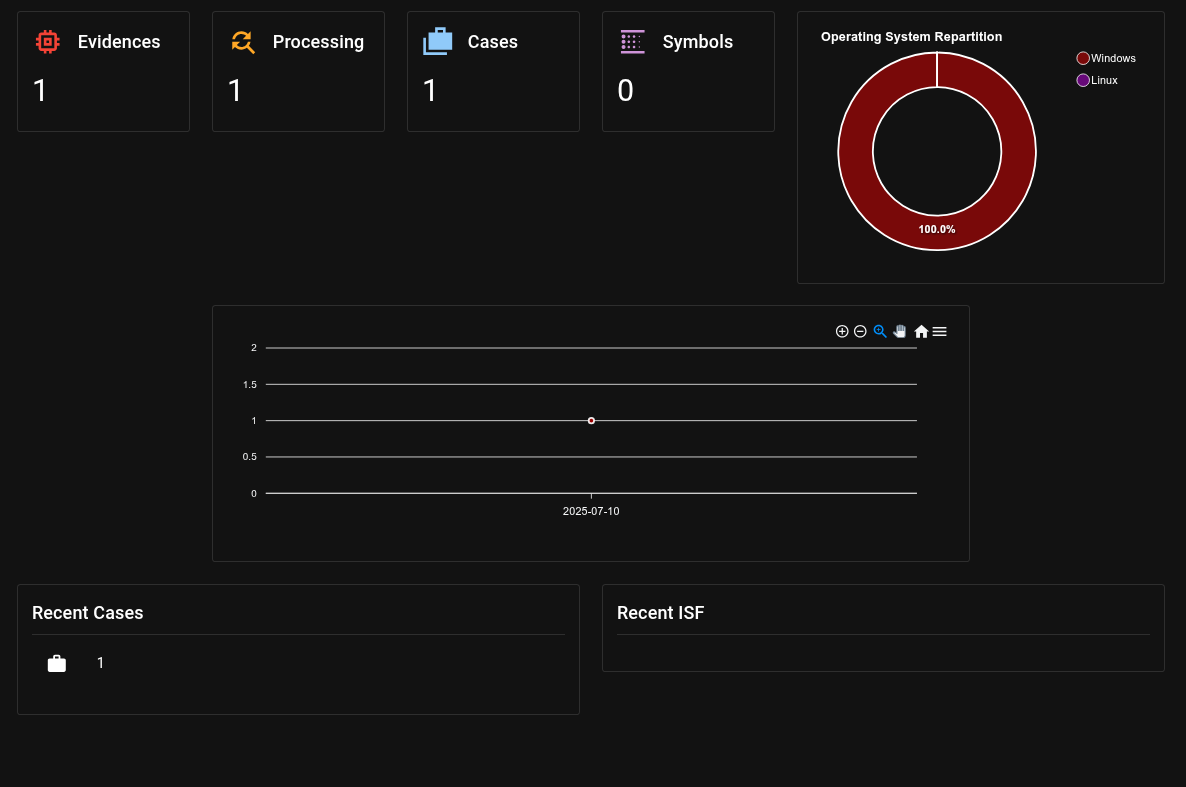
\includegraphics[width=1\linewidth]{images/volweb-original/volweb-dashboard.png}
\end{figure}

La navigazione segue una struttura gerarchica naturale: dalla lista dei casi si accede ai dettagli del singolo caso, da cui è possibile esplorare le evidenze associate e i risultati delle analisi. Questa struttura, apparentemente semplice, nasconde una considerevole complessità nell'orchestrazione dei componenti React che gestiscono lo stato dell'applicazione.

L'uso estensivo di feedback visivo mantiene l'utente informato sullo stato delle operazioni. Progress bar per upload e analisi, notifiche per il completamento di task e indicatori di stato per ogni componente contribuiscono a creare un'esperienza utente che minimizza l'incertezza e l'ansia tipiche delle operazioni di lunga durata.

\subsection{Visualizzazione dei risultati}

Uno dei maggiori punti di forza di VolWeb rispetto all’uso diretto di Volatility è la presentazione dei risultati: al posto di output testuali densi e poco leggibili, i dati vengono trasformati in visualizzazioni interattive che semplificano l’individuazione di anomalie e pattern sospetti.
Questa fase rappresenta anche una delle sfide principali del design di VolWeb: i plugin di Volatility generano output molto eterogenei, che spaziano da semplici liste a strutture dati complesse. Per affrontare questa varietà, VolWeb integra renderer dedicati ai tipi di dati più ricorrenti, in grado di tradurre automaticamente le tabelle testuali in visualizzazioni interattive.

\subsubsection{Visualizzazione dei processi}

La vista dei processi utilizza una rappresentazione ad albero che mostra chiaramente le relazioni parent-child tra processi. I processi orfani o con parent inusuali sono evidenziati visualmente, permettendo l'identificazione rapida di potenziali indicatori di compromissione. Ogni nodo dell'albero è espandibile per rivelare dettagli aggiuntivi come PID, tempo di creazione, numero di thread e handle, e spazio di memoria utilizzato.

\begin{figure}[H]
    \centering
    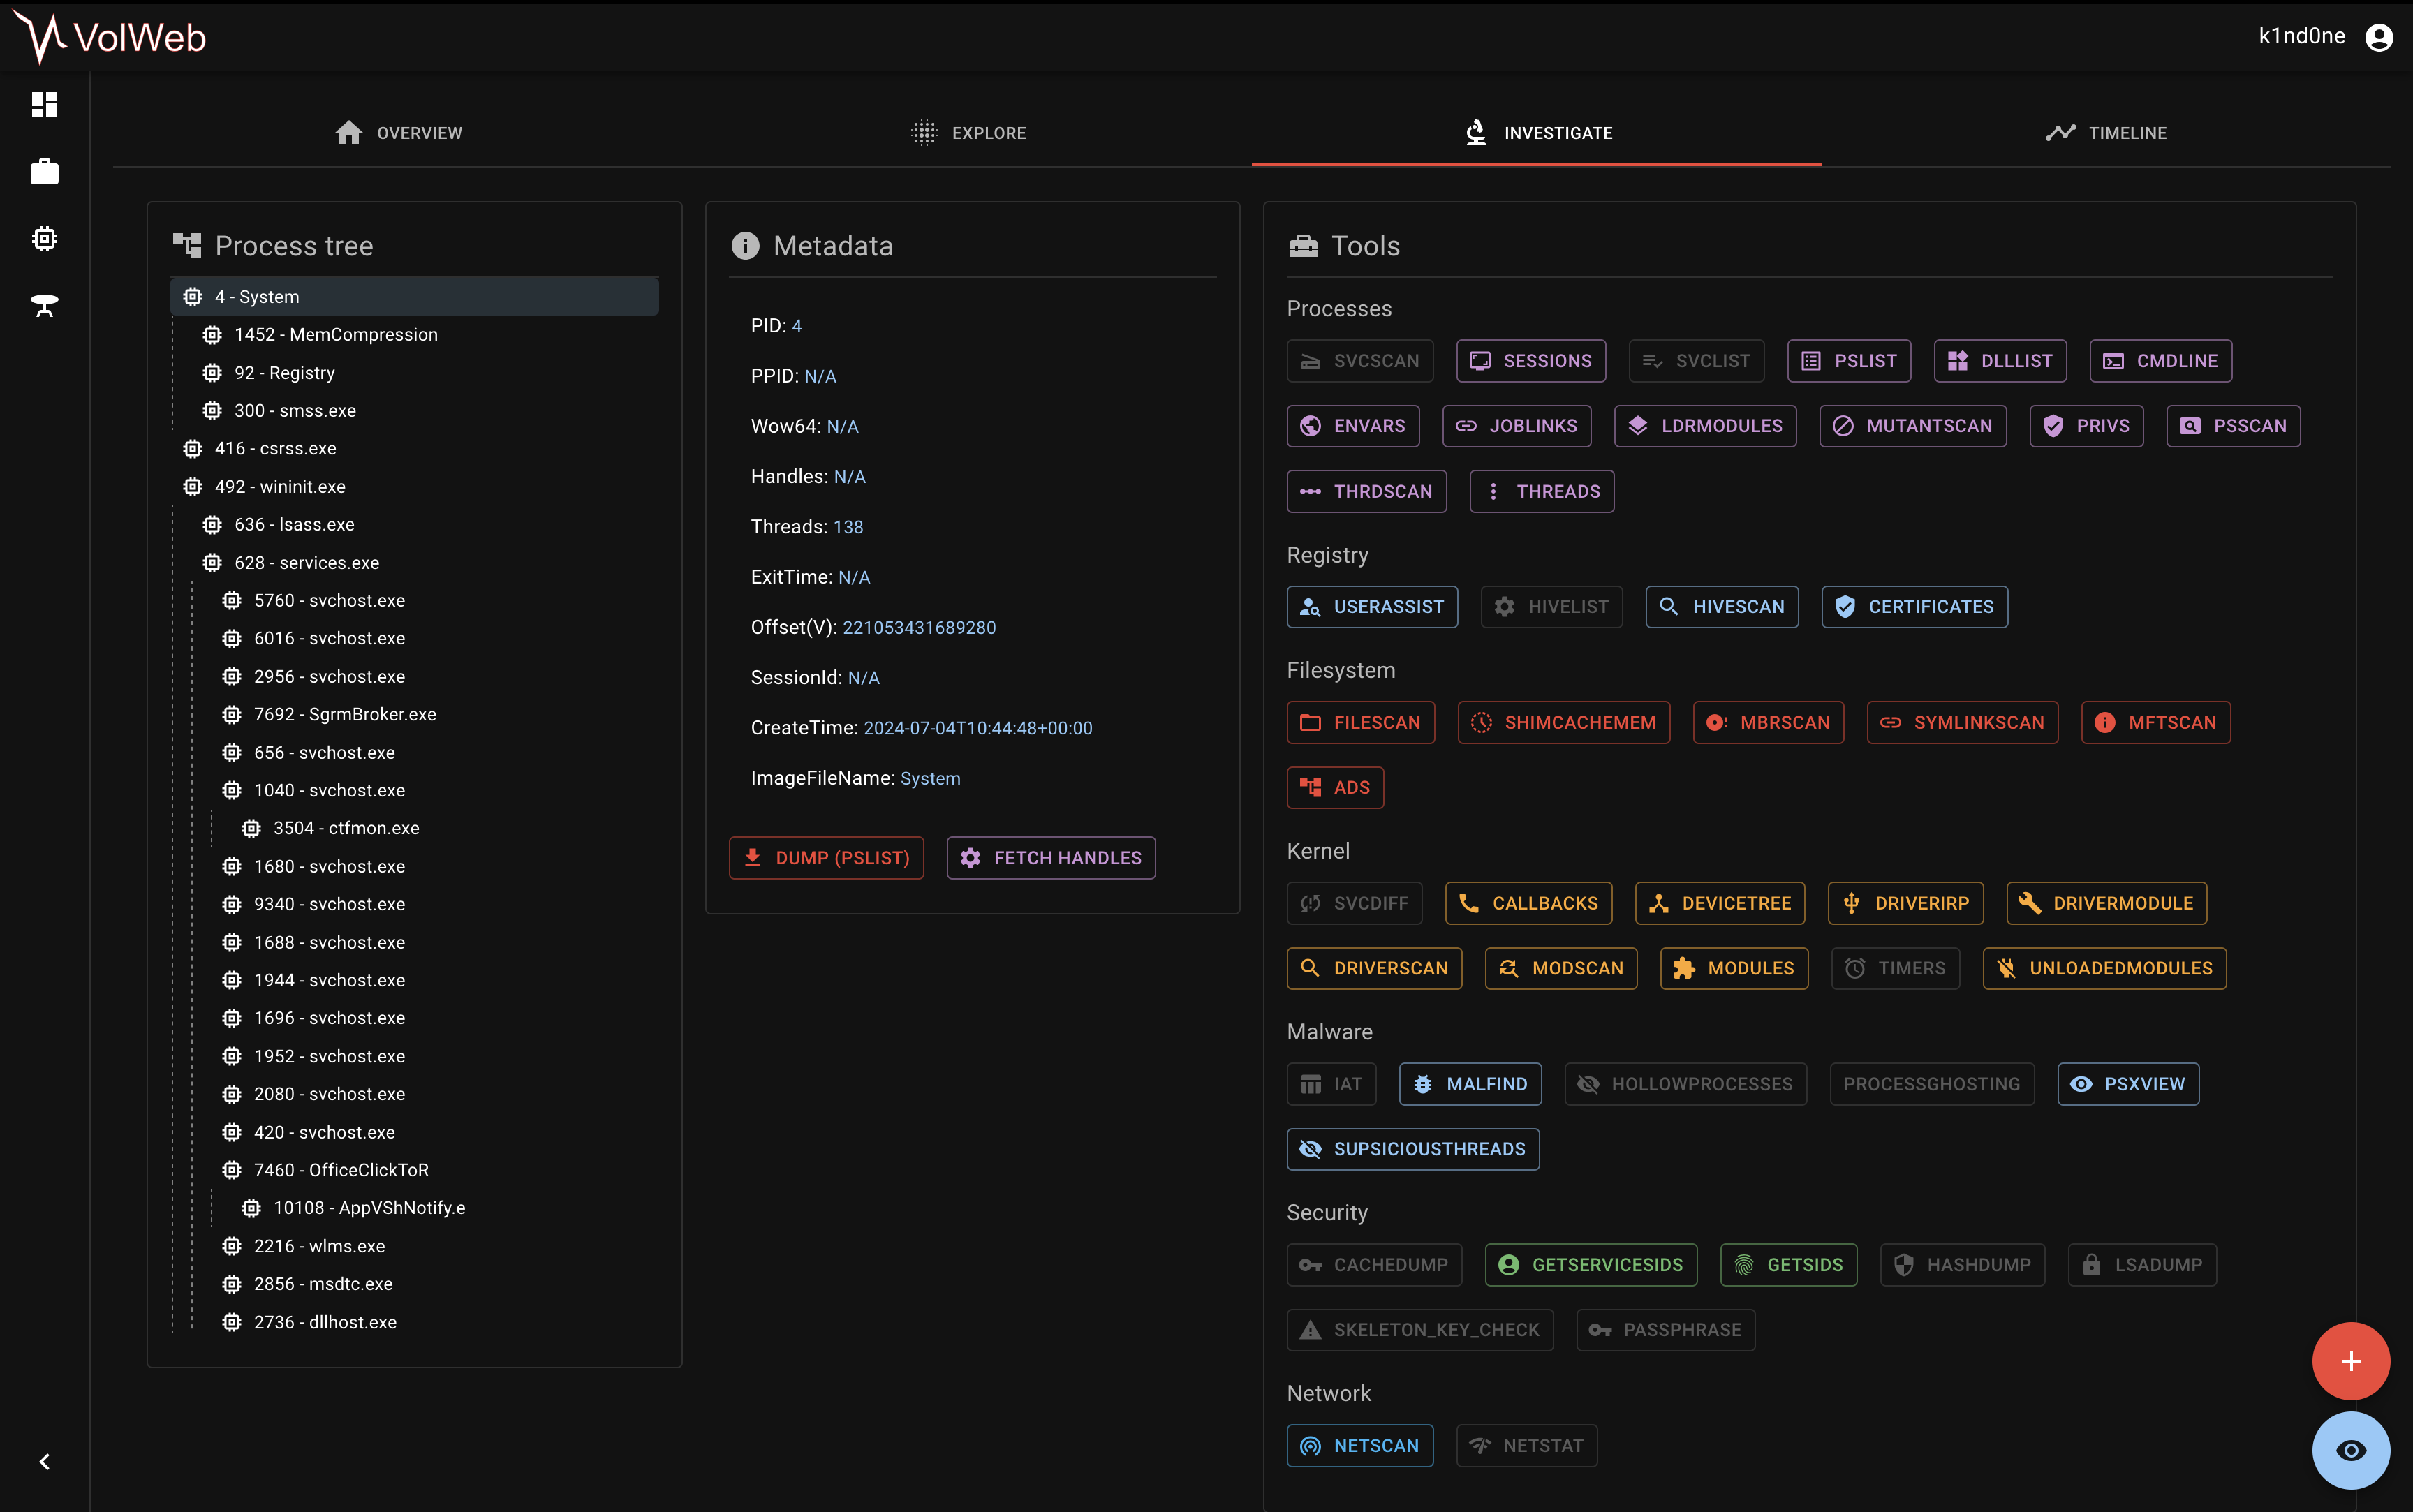
\includegraphics[width=1\linewidth]{images/volweb-original/volweb-process-tree.png}
\end{figure}

Per i dati di processo, il sistema presenta una vista tabellare arricchita che permette sorting, filtering e ricerca full-text. Ogni processo è cliccabile per accedere a una vista dettagliata che aggrega informazioni da multipli plugin correlati. Questa aggregazione, invisibile all'utente, richiede una logica complessa per correlare dati provenienti da plugin diversi basandosi su identificatori comuni come PID e offset di memoria.

\subsubsection{Visualizzazione delle connessioni di rete}

Per le connessioni di rete, VolWeb offre multiple viste complementari. La vista tabellare fornisce tutti i dettagli tecnici: processo proprietario, protocollo, indirizzi IP e porte locali e remote, stato della connessione. La vista grafica, basata su D3.js, visualizza le connessioni come un grafo interattivo dove i nodi rappresentano processi ed endpoint, mentre gli archi indicano le connessioni attive.

\begin{figure}[H]
    \centering
    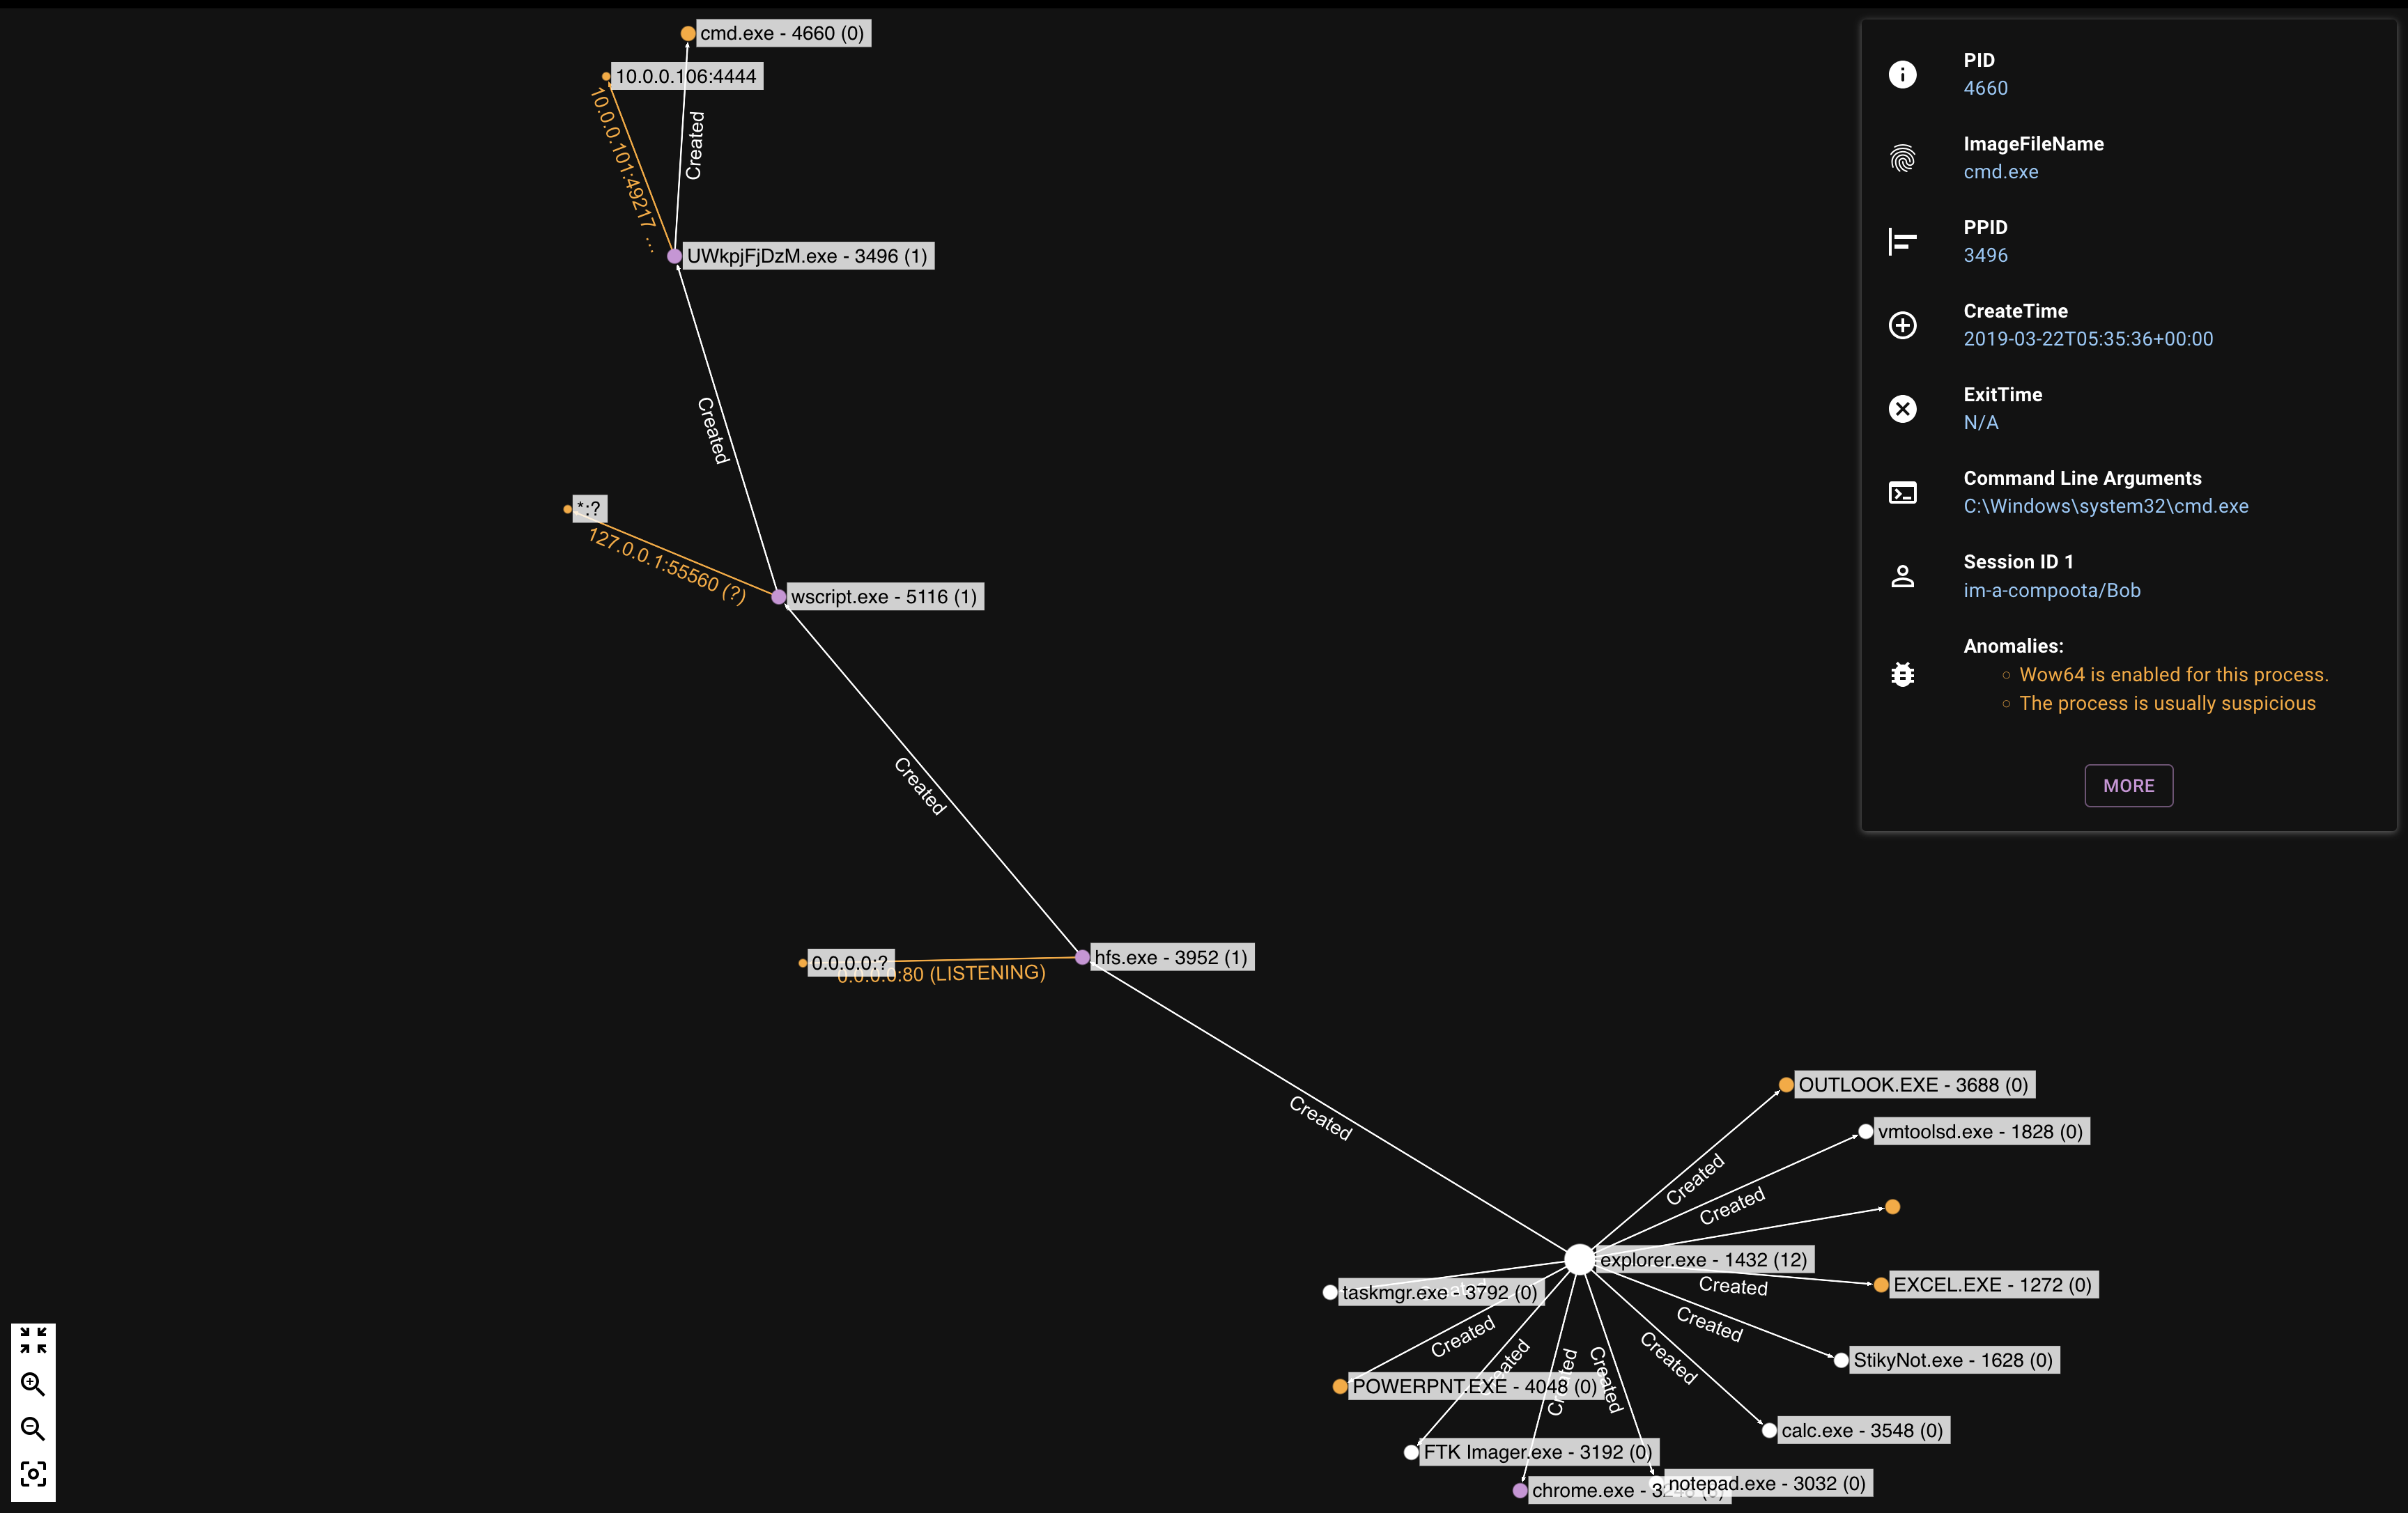
\includegraphics[width=0.9\linewidth]{images/volweb-original/volweb-network-graph.png}
\end{figure}

Le informazioni di rete sono presentate attraverso una combinazione di viste tabellari e visualizzazioni grafiche. La vista tabellare permette un'analisi dettagliata di ogni connessione, mentre la visualizzazione grafica offre una comprensione immediata delle relazioni tra processi e endpoint remoti.

\subsubsection{Sistema di ricerca}

Con dump di memoria che possono contenere informazioni su centinaia di processi e migliaia di artefatti, la capacità di ricerca efficace diventa critica. VolWeb implementa un motore di ricerca che supporta query sia semplici che complesse, permettendo agli analisti di trovare rapidamente informazioni rilevanti. La ricerca full-text opera su tutti i campi dei risultati, permettendo di trovare rapidamente riferimenti a file specifici, indirizzi IP, o stringhe sospette. Il sistema supporta inoltre filtering avanzato per tipo di dato, permettendo per esempio di visualizzare solo i processi che hanno connessioni di rete attive o solo le DLL caricate da percorsi non standard.

\section{Funzionalità Principali}

\subsection{Sistema di Plugin e Estensibilità}

VolWeb implementa un sistema di plugin che riflette e estende quello di Volatility. Ogni plugin supportato è rappresentato da una configurazione che specifica parametri, dipendenze e modalità di visualizzazione dei risultati. Questa architettura permette di aggiungere supporto per nuovi plugin di Volatility senza modifiche al core dell'applicazione.

L'esecuzione dei plugin avviene attraverso Celery task che permettono parallelizzazione e gestione robusta degli errori. Quando un utente richiede l'esecuzione di un'analisi, VolWeb crea un task Celery per ogni plugin selezionato. Questi task vengono distribuiti ai worker disponibili, permettendo l'esecuzione parallela su hardware multi-core o distribuito.

L'orchestrazione dei plugin tiene conto delle dipendenze tra di essi. Alcuni plugin richiedono i risultati di altri per funzionare correttamente. VolWeb gestisce automaticamente queste dipendenze, assicurando che i plugin vengano eseguiti nell'ordine corretto e che i risultati siano disponibili quando necessario.

\subsection{API REST}

VolWeb espone una API REST completa che permette l'automazione e l'integrazione con altri strumenti. La documentazione delle API, generata automaticamente da Django REST Framework, fornisce dettagli su ogni endpoint disponibile, parametri richiesti e formato delle risposte.

\begin{figure}[H]
    \centering
    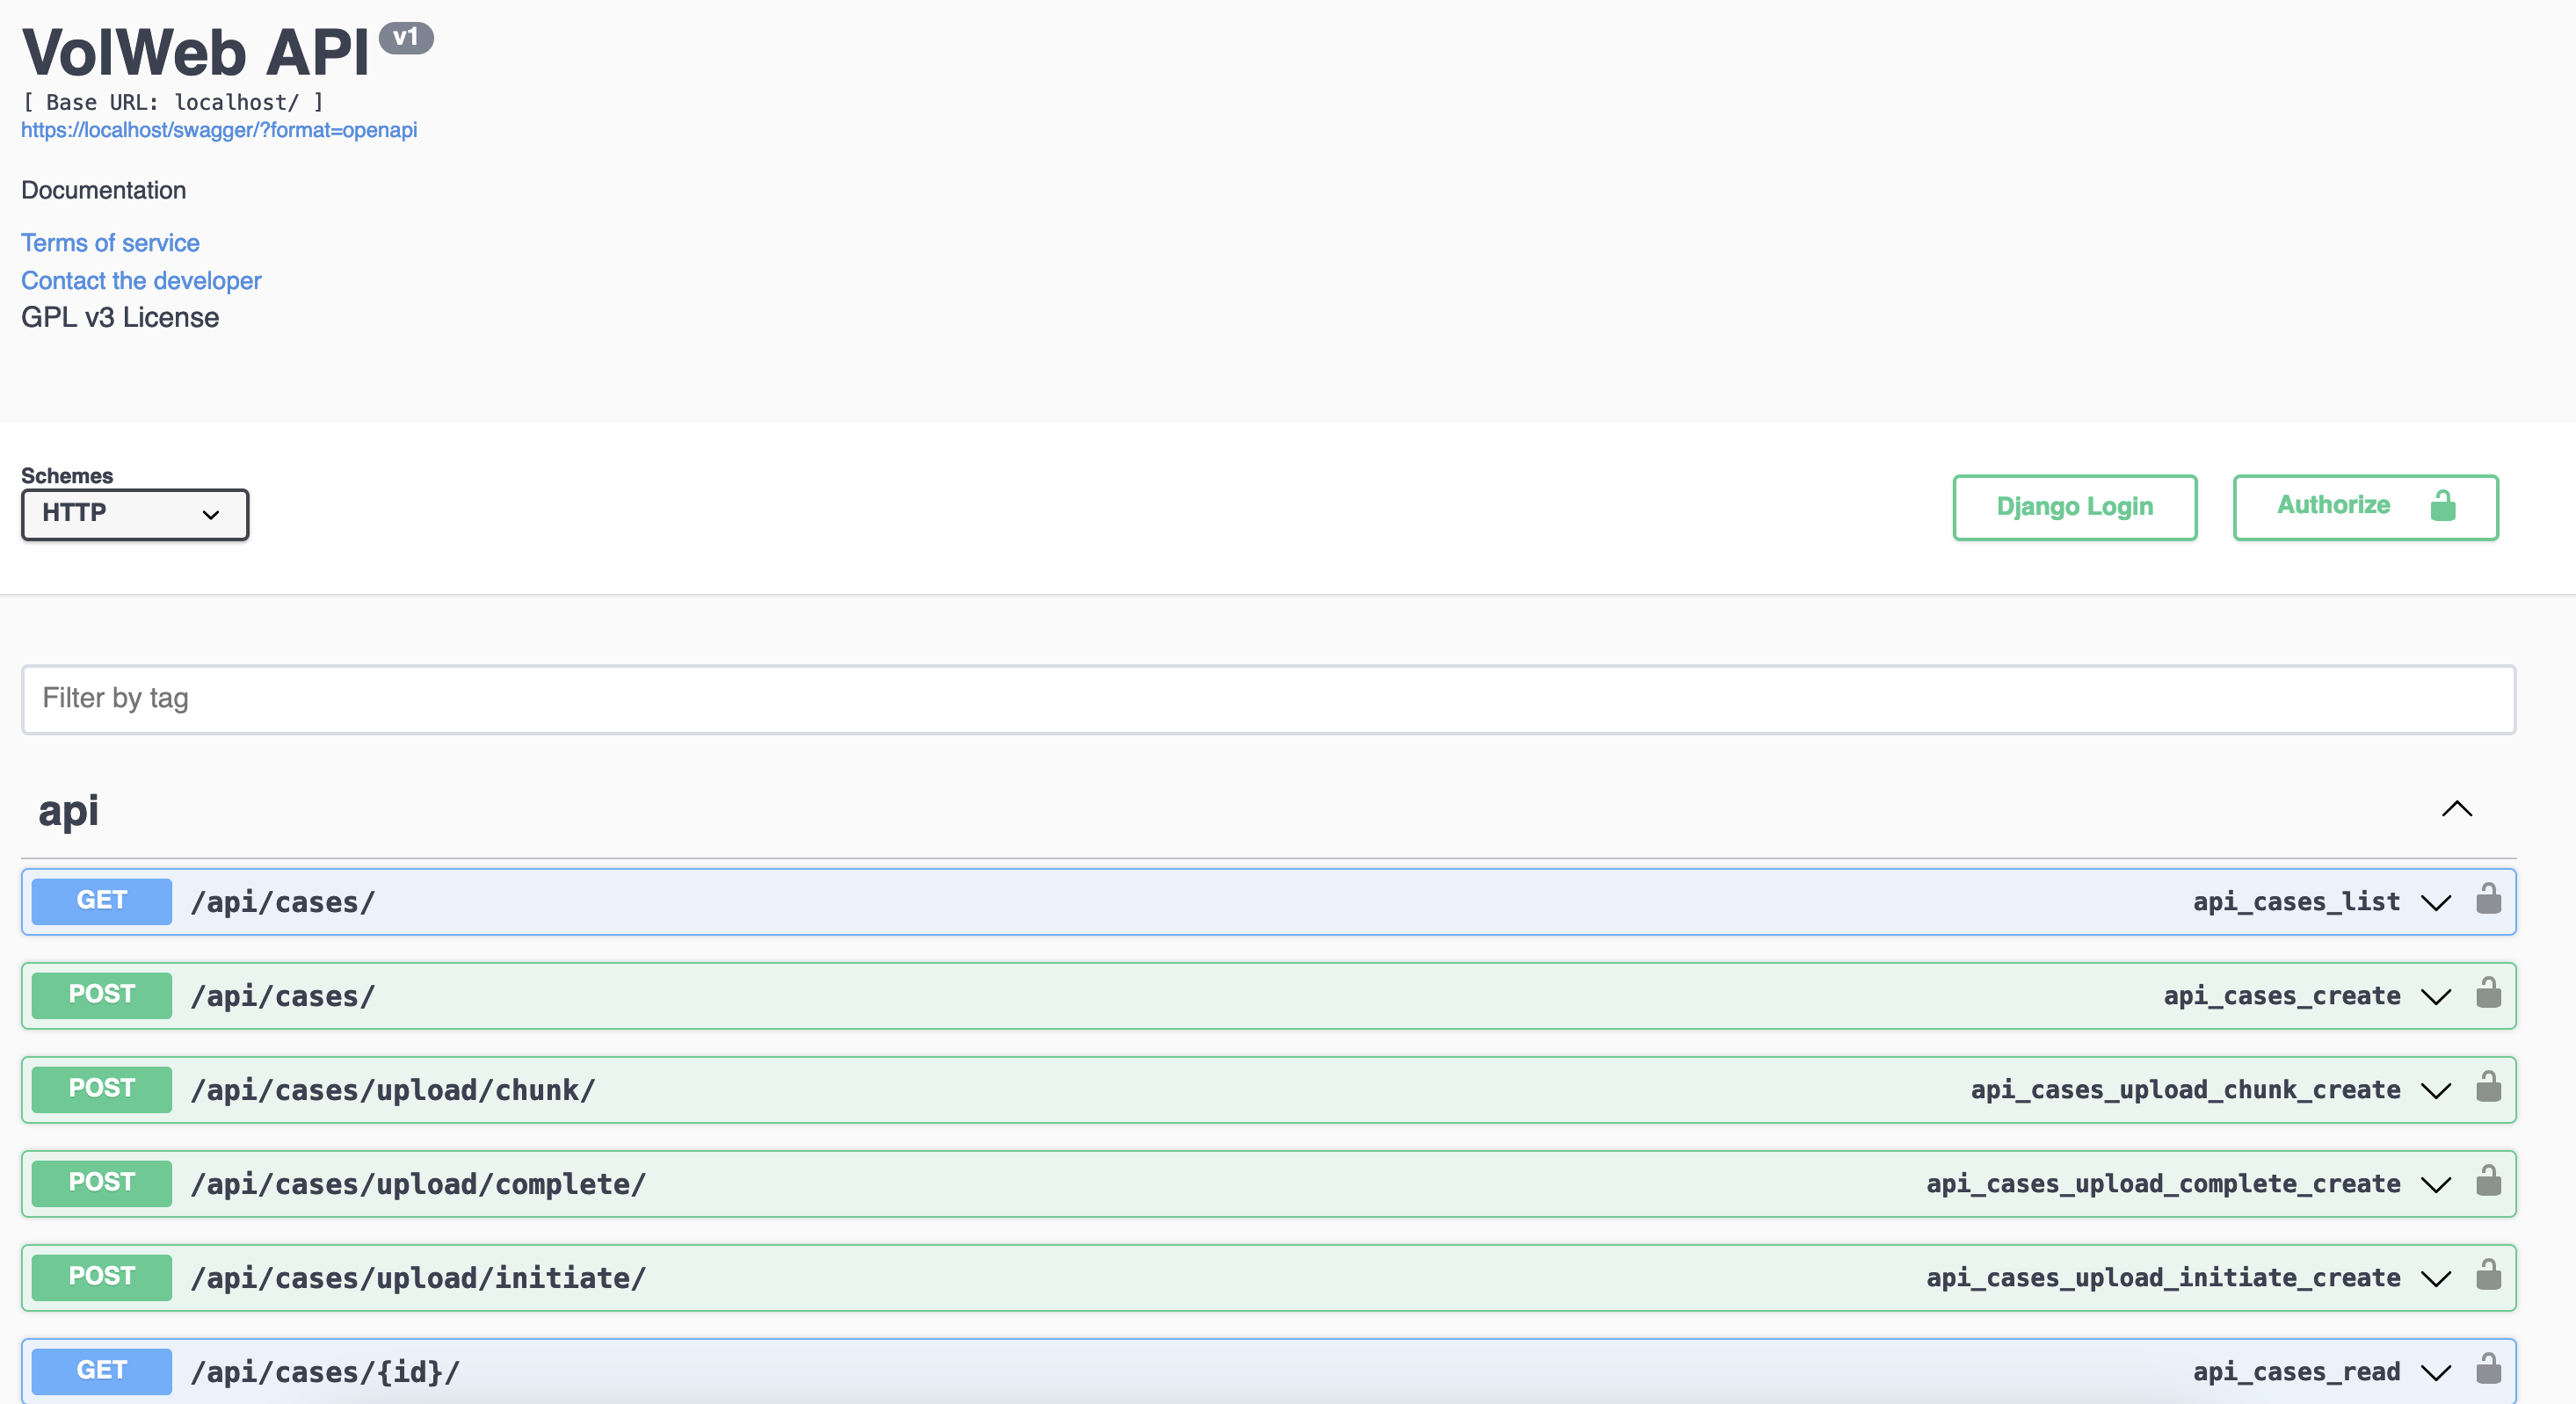
\includegraphics[width=1\linewidth]{images/volweb-original/volweb-swagger.png}
\end{figure}

Gli endpoint principali includono la gestione dei casi con creazione, modifica e cancellazione, la gestione delle evidenze con upload, download e metadata, l'esecuzione dei plugin con selezione, parametrizzazione e monitoraggio, e il recupero dei risultati con filtering, paginazione ed export. Questa esposizione attraverso API standardizzate trasforma VolWeb in un componente integrabile in pipeline di analisi più ampie, permettendo l'automazione di workflow complessi.

\subsection{Sicurezza e Controllo degli Accessi}

La sicurezza in VolWeb è implementata a più livelli, partendo da un robusto sistema di autenticazione basato sul framework di Django. Gli utenti devono autenticarsi per accedere a qualsiasi funzionalità, e le sessioni sono gestite in modo sicuro con token che scadono dopo un periodo di inattività configurabile.

Il sistema di autorizzazione implementa un modello di permessi granulare. Gli utenti possono avere ruoli diversi con capacità appropriate: amministratori con accesso completo, analisti con capacità di creare e gestire casi, e viewer con accesso in sola lettura. A livello di caso, è possibile definire permessi specifici, permettendo la condivisione selettiva di investigazioni tra team diversi mantenendo la segregazione di informazioni sensibili.

\section{Limitazioni e Considerazioni}

Nonostante le capacità significative, la versione originale di VolWeb presenta alcune limitazioni importanti. L'assenza di supporto per YARA rappresenta probabilmente la mancanza più significativa, limitando le capacità di threat hunting della piattaforma. Questa limitazione impedisce l'implementazione di capacità di pattern matching avanzate necessarie per identificare minacce custom o varianti di malware conosciuti, una funzionalità critica in contesti operativi moderni dove le minacce evolvono rapidamente.

Mentre VolWeb presenta i risultati in modo organizzato, manca di capacità avanzate di correlazione tra risultati di plugin che potrebbero identificare automaticamente pattern sospetti attraverso dataset diversi. Questa limitazione richiede che l'analista mantenga mentalmente le correlazioni, aumentando il carico cognitivo durante investigazioni complesse.

L'integrazione con threat intelligence esterna è assente. In un panorama dove la condivisione di IOC e intelligence è fondamentale, l'impossibilità di importare automaticamente feed di threat intelligence o di arricchire i risultati con contesto esterno rappresenta una limitazione operativa significativa. Gli analisti devono manualmente correlare gli artefatti con informazioni esterne, rallentando il processo investigativo.

Nonostante i significativi progressi rappresentati da VolWeb nella democratizzazione dell'accesso alla memory forensics, è stata l'esperienza operativa in contesti ad alta intensità a evidenziare le aree di miglioramento più critiche. Il capitolo seguente analizza come l'esercitazione NATO Locked Shields 2025 abbia fornito il banco di prova ideale per identificare i requisiti che hanno guidato l'espansione presentata in questa tesi.
\chapter{NATO CCDCOE Locked Shields}

L'esercitazione Locked Shields \cite{ccdcoe2025} rappresenta il principale banco di prova internazionale per le capacità di cyber defense, dove le competenze teoriche si confrontano con la complessità operativa della sicurezza informatica moderna. Il presente capitolo analizza il contesto distintivo di questa esercitazione, con particolare attenzione al ruolo dell'analisi forense digitale e ai requisiti emersi dall'edizione 2025 che hanno motivato lo sviluppo delle espansioni di VolWeb oggetto di questa tesi.

\section{Descrizione dell'Esercitazione}

\subsection{Storia e obiettivi di Locked Shields}

Locked Shields costituisce la più estesa e articolata esercitazione di cyber defense a livello globale, organizzata annualmente dal NATO Cooperative Cyber Defence Centre of Excellence (CCDCOE) con sede a Tallinn, Estonia. Concepita nel 2010 come risposta diretta agli attacchi cibernetici del 2007 contro l'Estonia, l'esercitazione ha conosciuto una crescita esponenziale: da evento regionale con limitata partecipazione si è trasformata in un'esercitazione di portata globale che coinvolge oltre 40 nazioni e più di 4000 specialisti del settore.

L'obiettivo principale di Locked Shields consiste nel fornire un ambiente simulato altamente realistico in cui team internazionali congiunti possano verificare e perfezionare le proprie competenze tecniche e procedurali in scenari di conflitto cibernetico su vasta scala. Diversamente dalle tradizionali competizioni Capture The Flag (CTF), che tendono a concentrarsi su sfide tecniche isolate, Locked Shields propone una simulazione integrata di warfare cibernetico, incorporando dimensioni tecniche, legali, di comunicazione strategica e cooperazione internazionale.

L'esercitazione si sviluppa attorno a uno scenario geopolitico fittizio ma verosimile, generalmente incentrato sulla nazione immaginaria di "Berylia", bersaglio di una campagna di attacchi cibernetici coordinati. I team partecipanti assumono il ruolo di difensori delle infrastrutture critiche beryliane - reti elettriche, sistemi idrici, telecomunicazioni, servizi finanziari e apparati militari - con il duplice obiettivo di respingere gli attacchi e garantire la continuità operativa dei servizi essenziali. Tale approccio multidimensionale rispecchia fedelmente la natura della cyber warfare contemporanea, caratterizzata non da incidenti isolati ma da campagne orchestrate finalizzate alla destabilizzazione sistemica.

L'evoluzione di Locked Shields ha seguito parallelamente la trasformazione del panorama delle minacce cibernetiche. Se le prime edizioni si focalizzavano prevalentemente su attacchi Distributed Denial of Service (DDoS) e defacement di siti web, le iterazioni più recenti hanno introdotto scenari di complessità crescente: Advanced Persistent Threats (APT), supply chain attacks, campagne ransomware coordinate e compromissioni di sistemi di controllo industriale (SCADA/ICS). L'edizione 2025 ha segnato un ulteriore salto qualitativo, introducendo per la prima volta scenari basati su attacchi potenziati dall'intelligenza artificiale e operazioni di disinformazione mediante deepfake, anticipando le minacce emergenti nel dominio cibernetico.

\subsection{Struttura della competizione}

Locked Shields adotta una struttura articolata che bilancia accuratamente realismo operativo e obiettivi formativi. L'esercitazione si sviluppa su tre giorni di intensa attività operativa, preceduti da un periodo preparatorio di diverse settimane.

\subsubsection{Fase preparatoria}
Il periodo pre-esercitazione riveste importanza cruciale per il successo dei team partecipanti. Durante questa fase, i team ottengono accesso limitato all'infrastruttura virtualizzata che dovranno successivamente difendere, permettendo loro di familiarizzare con l'architettura dei sistemi, identificare vulnerabilità preesistenti, implementare misure di hardening preventivo e sviluppare playbook operativi. L'infrastruttura simulata comprende tipicamente ambienti eterogenei e complessi: reti aziendali basate su Active Directory con servizi di posta elettronica e applicazioni web, sistemi di controllo industriale per la gestione di infrastrutture critiche simulate, portali di servizi pubblici inclusi sistemi di voto elettronico, e infrastrutture militari comprendenti sistemi C4ISR (Command, Control, Communications, Computers, Intelligence, Surveillance and Reconnaissance) supportati da reti 5G di nuova generazione.

I team partecipanti, denominati Blue Team, rappresentano il Rapid Reaction Team (RRT) nazionale di Berylia e devono strutturarsi in unità specializzate con competenze complementari: network defense, amministrazione sistemi Windows e Linux, sicurezza applicazioni web, gestione SIEM (Security Information and Event Management), analisi forense, consulenza legale, gestione mediatica e cyber intelligence.

\subsubsection{Fase esecutiva}
I tre giorni di esercitazione vera e propria vedono i Blue Team confrontarsi con ondate progressive di attacchi orchestrati dal Red Team, composto da esperti di penetration testing e cyber warfare provenienti dal CCDCOE e dalle nazioni partner. La progressione degli attacchi segue una narrativa coerente che simula l'escalation tipica di una campagna APT: dalla ricognizione iniziale alla compromissione sistemica.

Il Green Team garantisce il funzionamento dell'infrastruttura di simulazione e introduce elementi di complessità aggiuntiva mediante l'iniezione di eventi non direttamente correlati agli attacchi cibernetici, quali guasti hardware o richieste operative urgenti, incrementando il realismo dello scenario. Il White Team svolge funzioni di arbitraggio, valutando le prestazioni dei team secondo metriche predefinite e garantendo il rispetto delle regole di ingaggio.

La dimensione puramente tecnica rappresenta solo una componente della sfida. I team devono infatti produrre deliverable diversificati che riflettono la complessità della gestione di una crisi cibernetica reale: situation report per la catena di comando, comunicati stampa per la gestione dell'opinione pubblica, analisi legali delle opzioni di risposta disponibili, e raccomandazioni strategiche per i decisori politici.

\subsection{Scenari tipici e sfide tecniche}

Gli scenari proposti in Locked Shields sono progettati per verificare l'intero spettro delle capacità di cyber defense. L'edizione 2025 ha presentato sfide di complessità particolare, mettendo alla prova anche i team più esperti attraverso una combinazione di minacce tradizionali ed emergenti.

\paragraph{Advanced Persistent Threats}
I Red Team hanno simulato con accuratezza gruppi APT sponsorizzati da stati nazionali, replicandone fedelmente Tactics, Techniques and Procedures (TTP). Gli attacchi multi-stadio hanno incluso campagne di spear-phishing con documenti malevoli altamente mirati, sfruttamento di vulnerabilità zero-day simulate ma realistiche, movimenti laterali mediante tecniche living-off-the-land che abusano di strumenti legittimi del sistema, esfiltrazione di dati attraverso canali covert difficilmente rilevabili, e deployment di ransomware come cortina fumogena per mascherare operazioni di spionaggio più sofisticate.

\paragraph{Supply Chain Attacks}
Ispirandosi a incidenti reali come il caso SolarWinds, gli scenari hanno incorporato compromissioni della catena di approvvigionamento software attraverso vettori multipli: meccanismi di aggiornamento compromessi per la distribuzione capillare di malware, librerie di terze parti contenenti backdoor accuratamente camuffate, compromissione di fornitori VPN per garantire accesso persistente alle reti target, e manipolazione del firmware di dispositivi di rete critici.

\paragraph{Attacchi a sistemi OT}
La compromissione di sistemi SCADA/ICS ha testato le capacità di protezione delle infrastrutture critiche simulate. Gli scenari hanno incluso manipolazione di Programmable Logic Controller (PLC) per indurre malfunzionamenti controllati, attacchi mirati a protocolli industriali specifici come Modbus e DNP3, deployment di ransomware ottimizzato per ambienti OT con logiche di propagazione specifiche, e tentativi di compromissione dei sistemi di sicurezza che avrebbero potuto causare danni fisici nell'ambiente simulato.

\paragraph{Operazioni informative}
L'edizione 2025 ha posto particolare enfasi sulla dimensione informativa del conflitto cibernetico, introducendo: deepfake video raffiguranti leader governativi in dichiarazioni compromettenti, campagne di disinformazione sincronizzate con gli attacchi tecnici per massimizzare l'impatto psicologico, operazioni hack-and-leak mirate a minare la fiducia pubblica nelle istituzioni, e manipolazione coordinata dei social media per amplificare percezioni di crisi.

\paragraph{Vettori di attacco innovativi}
L'innovazione continua negli scenari di attacco ha incluso: malware dotato di capacità di intelligenza artificiale per l'adattamento dinamico alle contromisure difensive, attacchi a infrastrutture cloud e ambienti containerizzati sempre più prevalenti, compromissione di dispositivi IoT per la creazione di botnet massive difficilmente neutralizzabili, e sfide legate all'implementazione di crittografia quantum-safe.

La complessità tecnica degli scenari è stata ulteriormente amplificata dal requisito di mantenere operativi i servizi essenziali durante gli attacchi, impedendo ai team di adottare approcci semplicistici basati sull'isolamento totale dei sistemi compromessi e richiedendo invece un bilanciamento continuo tra esigenze di sicurezza e disponibilità operativa.

\section{Ruolo del DFIR in Locked Shields}

\subsection{Importanza dell'analisi forense nelle CTF}

A differenza delle tradizionali competizioni CTF che privilegiano l'exploitation di vulnerabilità o la risoluzione di puzzle crittografici, Locked Shields attribuisce all'analisi forense digitale un ruolo centrale e distintivo. Tale scelta riflette la realtà operativa del mondo reale, dove la capacità di comprendere tempestivamente la natura, le modalità e le finalità di un attacco risulta spesso più determinante della prevenzione assoluta.

Nel contesto di Locked Shields 2025, l'attività forense si è configurata come una CTF di tipo Jeopardy quasi completamente autonoma rispetto alla rete di gioco principale di attacco e difesa. Questa struttura innovativa ha permesso ai team forensi di operare in un ambiente dedicato, affrontando 15 challenge specificamente progettate per testare diverse competenze investigative: 12 challenge di analisi post-mortem su dump di memoria e immagini disco, 2 challenge di analisi live su sistemi in esecuzione, e 1 challenge collaborativa da svolgere congiuntamente con i team Legal Advisor (LegAd) e Cyber Intelligence per la redazione di un report tecnico-legale integrato.

L'analisi forense in questo contesto ha svolto un ruolo multiplo e determinante per il successo complessivo del Blue Team. Ha permesso, innanzitutto, di attribuire le attività malevole e di comprendere le intenzioni degli attaccanti simulati: identificare chi fossero e quali obiettivi strategici stessero perseguendo ha dato modo ai team di anticipare le mosse successive, ottimizzando così l’allocazione delle risorse difensive. Lo studio dei pattern comportamentali e delle TTP adottate ha reso possibile distinguere tra operazioni di spionaggio, di sabotaggio o semplicemente di disruption, consentendo di modulare le contromisure in modo più efficace.

Un altro aspetto fondamentale è stata la rapida determinazione dell’ambito di compromissione. Comprendere con precisione quanto fosse estesa la violazione ha rappresentato un fattore cruciale per attuare decisioni di contenimento tempestive e mirate. La capacità di riconoscere la differenza tra un incidente isolato e una compromissione sistemica ha influito direttamente sulle strategie di risposta adottate.

Parallelamente, l’analisi dettagliata del malware e delle tecniche impiegate ha fornito preziose indicazioni sulle capacità offensive degli avversari simulati. Questa intelligence ha reso possibile l’adozione di contromisure calibrate e proporzionate alla minaccia. Non meno importante, soprattutto in scenari che prevedevano una possibile evoluzione verso risposte legali o diplomatiche, è stata la produzione di evidenze forensi adeguate agli standard probatori. Questo ha richiesto una particolare attenzione alla metodologia e alla documentazione, garantendo la solidità delle prove raccolte.

Il contesto altamente vincolato nel tempo di Locked Shields ha trasformato la tradizionale attività di DFIR — solitamente un processo metodico e sequenziale — in una vera e propria capacità operativa dinamica, fondata su decisioni rapide prese spesso sulla base di informazioni incomplete. Ciò ha imposto ai team l’adozione di strategie di triage aggressive e un ricorso intensivo ad automazione e strumenti di supporto, con l’obiettivo di massimizzare l’efficienza analitica e mantenere un vantaggio tattico rispetto alle minacce.


\subsection{Scenari di incident response}

Gli scenari forensi proposti in Locked Shields 2025 hanno coperto l'intero spettro delle sfide investigative moderne, con particolare enfasi sulla correlazione tra evidenze tecniche e implicazioni operative più ampie.

\paragraph{Challenge di analisi post-mortem}
Le 12 challenge di analisi post-mortem hanno presentato scenari progressivamente complessi che richiedevano l'applicazione di tecniche forensi avanzate su dump di memoria e immagini disco. I team hanno dovuto affrontare:
\begin{itemize}
    \item Identificazione di processi malevoli nascosti mediante tecniche di rootkit avanzate
    \item Ricostruzione di attività di esfiltrazione dati attraverso l'analisi di artefatti di rete in memoria
    \item Recupero di credenziali e chiavi crittografiche da processi in esecuzione
    \item Analisi di malware packed e offuscato presente solo in memoria
    \item Timeline reconstruction per determinare la sequenza esatta degli eventi di compromissione
    \item Identificazione di meccanismi di persistenza sofisticati implementati a livello kernel
    \item Estrazione di ioc da un dispositivo Android infetto e successivo reverse engineering di un apk malevolo
\end{itemize}

\paragraph{Challenge di analisi live}
Le 2 challenge di analisi live hanno richiesto l'investigazione di sistemi attivamente compromessi, ponendo sfide uniche in termini di preservazione delle evidenze e minimizzazione dell'impatto operativo:
\begin{itemize}
    \item Triage rapido di sistemi production critici senza causare interruzioni di servizio
    \item Identificazione e neutralizzazione di backdoor attive mantenendo l'accesso investigativo
    \item Monitoraggio real-time di attività malevole per comprendere obiettivi e metodologie
\end{itemize}

\paragraph{Challenge collaborativa tecnico-legale}
La challenge collaborativa ha rappresentato l'aspetto più innovativo e realistico del track forense. I team Forensics, LegAd e Cyber Intelligence hanno dovuto collaborare strettamente per produrre un report integrato che combinasse:
\begin{itemize}
    \item Analisi tecnica dettagliata degli indicatori di compromissione identificati
    \item Valutazione legale delle opzioni di risposta nel framework del diritto internazionale
    \item Assessment di intelligence sulle capacità e intenzioni degli attaccanti
    \item Raccomandazioni operative bilanciate tra esigenze tecniche, legali e strategiche
\end{itemize}

Questa struttura ha enfatizzato come, nel contesto reale, l'analisi forense non operi in isolamento ma debba integrarsi con considerazioni legali, diplomatiche e strategiche per supportare processi decisionali complessi.

\subsection{Metriche di valutazione}

Il sistema di valutazione adottato per il track forense in Locked Shields 2025 ha riflesso la multidimensionalità delle competenze richieste nel DFIR moderno, andando oltre la semplice correttezza tecnica per abbracciare aspetti processuali e strategici.

\paragraph{Metriche tecniche}
Le metriche tecniche hanno misurato l'efficacia nell'identificazione e analisi degli artefatti forensi:
\begin{itemize}
    \item Accuratezza nell'identificazione di Indicators of Compromise (IOC)
    \item Completezza nella ricostruzione della catena di eventi
    \item Precisione nell'attribuzione tecnica basata su TTP analysis
    \item Velocità di completamento delle challenge mantenendo standard qualitativi
\end{itemize}

\paragraph{Metriche processuali}
L'aderenza alle best practice forensi è stata valutata attraverso:
\begin{itemize}
    \item Documentazione della metodologia applicata e della chain of custody
    \item Riproducibilità delle analisi effettuate
    \item Gestione appropriata delle evidenze digitali
    \item Qualità della documentazione prodotta
\end{itemize}

\paragraph{Metriche collaborative}
La challenge integrata ha introdotto metriche specifiche per la collaborazione interdisciplinare:
\begin{itemize}
    \item Integrazione efficace tra componenti tecniche e legali del report
    \item Coerenza tra findings forensi e valutazioni di intelligence
    \item Chiarezza comunicativa per audience non tecniche
    \item Tempestività nella produzione del report integrato
\end{itemize}

Il sistema di scoring ha deliberatamente enfatizzato non solo la correttezza tecnica ma anche la capacità di contestualizzare i findings forensi nel più ampio scenario operativo, riflettendo l'evoluzione del ruolo del DFIR da funzione puramente tecnica a componente strategica della cyber defense.

\section{Requisiti specifici per Locked Shields 2025}

\subsection{Analisi delle esigenze identificate}

L'esperienza maturata durante Locked Shields 2025 ha evidenziato requisiti operativi specifici che gli strumenti di analisi forense tradizionali faticano a soddisfare nel contesto di esercitazioni ad alta intensità e, per estensione, in scenari operativi reali caratterizzati da pressione temporale estrema.

\paragraph{Velocità di analisi e scalabilità}
Il formato Jeopardy del track forense, con 15 challenge da completare in tempo limitato, ha posto l'accento sulla necessità di strumenti capaci di processare rapidamente grandi volumi di dati mantenendo accuratezza analitica. La capacità di analizzare molteplici dump di memoria di circa 20 GB ciascuno in tempi stringenti è diventata requisito fondamentale, richiedendo elaborazione parallela di multiple evidenze per massimizzare il throughput analitico. Questo implica la necessità di meccanismi di triage automatico che identificano rapidamente artefatti ad alta priorità e sistemi di caching intelligente per ottimizzare analisi iterative, evitando la ripetizione di operazioni computazionalmente intensive.

\paragraph{Pattern matching e threat hunting avanzati}
La complessità del malware presentato nelle challenge ha evidenziato come le semplici signature statiche siano ormai inadeguate. Il supporto per regole YARA complesse con logiche condizionali sofisticate è emerso come requisito critico, accompagnato dalla necessità di identificare varianti e mutazioni di malware noti attraverso matching fuzzy e analisi comportamentale. La correlazione automatica di pattern attraverso evidenze multiple e la generazione assistita di nuove regole basata su campioni identificati rappresentano capacità essenziali per mantenere il passo con l'evoluzione delle minacce.

\paragraph{Integrazione e correlazione di evidenze eterogenee}
La necessità di correlare informazioni provenienti da dump di memoria, immagini disco e analisi live ha sottolineato l'importanza di piattaforme veramente integrate. Un formato dati unificato che permetta l'aggregazione di risultati da fonti diverse, timeline correlate che integrino eventi da molteplici sorgenti, e capacità di cross-reference automatico tra artefatti correlati sono diventati requisiti imprescindibili. Le visualizzazioni unificate devono presentare una vista olistica dell'incidente, permettendo agli analisti di comprendere rapidamente relazioni complesse tra evidenze diverse.

\paragraph{Collaborazione e knowledge sharing}
La challenge collaborativa tecnico-legale ha evidenziato come il DFIR moderno richieda stretta cooperazione tra specialisti di domini diversi. Workspace condivisi per analisi collaborative in tempo reale, meccanismi strutturati di annotazione e tagging per facilitare la comunicazione interdisciplinare, template integrati per la produzione di report che soddisfino requisiti tecnici e legali, e integration points con piattaforme di cyber threat intelligence sono emersi come requisiti fondamentali per supportare questa nuova modalità operativa.

\subsection{Gap tra strumenti esistenti e requisiti}

L'analisi comparativa tra i requisiti identificati e le capacità degli strumenti esistenti ha rivelato gap significativi che limitano l'efficacia operativa nel contesto di `Locked Shields` e scenari simili.

\paragraph{Volatility Framework: completezza analitica vs. efficienza operativa}
Nonostante Volatility rimanga il riferimento per la completezza delle capacità analitiche, le sue limitazioni in contesti time-critical sono emerse con chiarezza. L'architettura monolitica e l'elaborazione sequenziale si sono rivelate inadeguate per l'analisi rapida di dump multipli. L'interfaccia a riga di comando, per quanto potente per utenti esperti, rallenta significativamente il processo di triage iniziale quando ogni minuto conta. L'output testuale non strutturato richiede post-processing manuale intensivo per identificare informazioni rilevanti, mentre l'integrazione limitata con YARA impedisce ricerche complesse basate su pattern comportamentali. L'assenza di funzionalità collaborative native rappresenta un ulteriore ostacolo in contesti dove il lavoro di team è essenziale.

\paragraph{Soluzioni commerciali: user experience vs. flessibilità}
Gli strumenti commerciali come Magnet AXIOM e Mandiant Redline, pur offrendo interfacce più intuitive, presentano limitazioni critiche in contesti competitivi. I modelli di licensing restrittivi limitano l'accesso simultaneo necessario per team numerosi o di natura nojn prettamente enterprise, mentre le capacità di customizzazione limitate impediscono l'implementazione rapida di nuove tecniche analitiche richieste da scenari in evoluzione. La natura proprietaria di questi strumenti preclude estensioni o modifiche per requisiti specifici, riducendone l'utilità in contesti che richiedono adattabilità estrema.

\paragraph{Frammentazione dell'ecosistema}
L'assenza di standard condivisi e l'incompatibilità tra strumenti creano inefficienze sistemiche che si amplificano sotto pressione temporale. La necessità di utilizzare tool multipli per coprire l'intero spettro di requisiti introduce overhead significativo nel trasferimento di dati e contesto. La duplicazione di effort analitico dovuta a incompatibilità di formati, la difficoltà nel mantenere una vista unificata dell'investigazione, e la complessità nella gestione della chain of custody attraverso tool eterogenei rappresentano ostacoli operativi significativi che possono compromettere l'efficacia complessiva dell'analisi.

\subsection{Opportunità di miglioramento}

L'identificazione dei gap ha delineato opportunità concrete per l'evoluzione degli strumenti di analisi forense, con particolare riferimento all'integrazione di capacità avanzate in piattaforme unificate come VolWeb.

\paragraph{Architettura modulare e scalabile}
L'adozione di un'architettura basata su microservizi emerge come risposta naturale alle sfide identificate. La scalabilità orizzontale permette di gestire i carichi di lavoro variabili tipici delle esercitazioni, mentre l'isolamento dei componenti garantisce resilienza e manutenibilità. La possibilità di ottimizzare indipendentemente componenti critici per le performance, combinata con la facilità di integrazione di nuove funzionalità senza impatti sistemici, crea una piattaforma evolutiva capace di adattarsi a requisiti in continua evoluzione.

\paragraph{Integrazione nativa di capacità di pattern matching}
L'incorporazione profonda di YARA e tecnologie similari rappresenta un'opportunità trasformativa per l'efficacia investigativa. Un editor integrato per creazione e testing di regole con validazione in tempo reale può drammaticamente accelerare lo sviluppo di nuove detection. Ottimizzazioni specifiche per lo scanning di memoria, gestione efficiente di dataset di grandi dimensioni, e capacità di correlazione cross-evidenza per identificare pattern distribuiti possono moltiplicare l'efficacia analitica. L'applicazione di tecniche di machine learning per suggerire regole basate su nuovi campioni rappresenta la frontiera futura del pattern matching automatizzato.

\paragraph{Interfacce collaborative e knowledge management}
Il supporto nativo per workflows collaborativi può trasformare radicalmente l'efficacia dei team forensi. Workspace condivisi con sincronizzazione real-time permettono a specialisti diversi di lavorare simultaneamente sulla stessa evidenza, mentre template di report integrati assicurano che i risultati siano comunicati efficacemente a stakeholder tecnici, legali ed executive. L'integrazione con piattaforme di Threat Intelligence come MISP e OpenCTI, combinata con audit trail completi per requisiti di compliance, crea un ecosistema integrato che supporta l'intero ciclo di vita dell'investigazione.

\paragraph{Automazione context-aware}
L'implementazione di automazione intelligente rappresenta la chiave per gestire la complessità crescente mantenendo tempi di risposta rapidi. Pipeline di pre-processing che identificano e prioritizzano evidenze critiche possono ridurre drasticamente il tempo necessario per il triage iniziale. Classificatori basati su machine learning per la categorizzazione automatica di processi e comportamenti, combinati con la generazione automatica di IOC con confidence scoring, permettono agli analisti di concentrarsi sugli aspetti più critici dell'investigazione. L'orchestrazione di analisi complesse attraverso playbook personalizzabili standardizza le best practice mantenendo la flessibilità necessaria per scenari non standard.

Queste opportunità di miglioramento non rappresentano mere ottimizzazioni incrementali, ma trasformazioni fondamentali necessarie per colmare il divario tra le capacità attuali e i requisiti operativi emersi da contesti ad alta intensità come Locked Shields. La loro implementazione in piattaforme integrate come VolWeb può significativamente elevare le capacità di risposta della comunità DFIR di fronte a minacce sempre più sofisticate.

Tra le diverse opportunità identificate, l'integrazione del supporto YARA in VolWeb è emersa come priorità immediata per diverse ragioni convergenti. La centralità del pattern matching nelle challenge forensi di Locked Shields 2025, combinata con la maturità tecnologica di YARA, ha reso questa integrazione il punto di partenza naturale per l'evoluzione della piattaforma. Inoltre, il supporto YARA rappresenta un enabler fondamentale per molte delle altre capacità identificate: l'automazione del threat hunting, la generazione di IOC, e la correlazione cross-evidenza dipendono tutte da robuste capacità di pattern matching. Pertanto, il lavoro di tesi si è concentrato prioritariamente sull'implementazione di un sistema completo di gestione, validazione ed esecuzione di regole YARA all'interno di VolWeb, ponendo le basi per future espansioni che potranno costruire su questa fondazione.

I requisiti emersi da Locked Shields 2025 hanno delineato una roadmap chiara per l'evoluzione di VolWeb. Il prossimo capitolo presenta l'analisi dettagliata, la progettazione e l'implementazione delle espansioni YARA, mostrando come queste trasformino VolWeb da strumento di visualizzazione a piattaforma completa per il threat hunting avanzato.
\chapter{Analisi e Progettazione delle Espansioni}

L'esperienza maturata durante l'esercitazione Locked Shields 2025 ha fornito insight fondamentali per guidare l'evoluzione di VolWeb. L'utilizzo della piattaforma in un contesto operativo ad alta pressione ha evidenziato sia i punti di forza che le limitazioni dell'implementazione originale, fornendo una roadmap chiara per le espansioni necessarie.

Durante Locked Shields, la necessità di analizzare rapidamente dump di memoria per identificare indicatori di compromissione ha reso evidente l'assenza di capacità di pattern matching avanzato. Gli analisti erano costretti a fare affidamento esclusivamente sui plugin predefiniti di Volatility, limitando significativamente la capacità di identificare minacce custom o varianti di malware conosciuti. Questa limitazione operativa ha motivato l'integrazione di YARA come priorità principale per le espansioni di VolWeb.

\section{Analisi dei Requisiti}

\subsection{Studio delle limitazioni di VolWeb originale}

L'analisi delle limitazioni di VolWeb è stata condotta attraverso tre prospettive complementari: l'esperienza diretta durante Locked Shields 2025, l'analisi del codice sorgente della versione originale, e il feedback raccolto dalla community degli utilizzatori.

Durante l'esercitazione Locked Shield, diverse limitazioni sono emerse con particolare evidenza. La più critica riguardava l'assenza di supporto per YARA, che impediva l'implementazione di capacità di threat hunting proattive. In uno scenario dove i red team utilizzavano malware custom e tecniche di evasione sofisticate, la capacità di definire e applicare pattern di ricerca specifici sarebbe stata fondamentale per l'identificazione rapida delle compromissioni.

L'architettura di autenticazione originale, basata su JWT e sessioni utente persistenti, si è rivelata un overhead non necessario nel contesto di deployment isolati tipici degli ambienti di analisi forense. Durante Locked Shields, dove ogni blue team operava in un ambiente segregato, la gestione degli utenti e delle sessioni aggiungeva complessità senza fornire valore reale. Questa osservazione ha portato alla decisione di semplificare l'architettura rimuovendo il layer di autenticazione nelle espansioni.

Similmente, il supporto per cloud storage (S3) presente nella versione originale si è dimostrato non necessario e potenzialmente problematico dal punto di vista della sicurezza. In ambienti forensi, dove i dump di memoria contengono dati estremamente sensibili, l'upload su storage cloud introduce rischi di data exfiltration e compliance. Durante Locked Shield, tutti i team hanno utilizzato esclusivamente storage locale, confermando che il supporto cloud non era una priorità per il target audience di VolWeb.

Un aspetto critico emerso durante l'esercitazione riguarda la resilienza dell'infrastruttura in scenari di cyber warfare simulato. Durante Locked Shields, i servizi cloud erano tra i primi target degli attacchi del red team, rendendo potenzialmente inaccessibili le evidenze archiviate remotamente proprio nel momento di maggior necessità. Questa esperienza ha confermato che affidarsi a storage cloud per evidenze forensi critiche introduce un single point of failure inaccettabile. In uno scenario reale di incident response, dove l'infrastruttura aziendale potrebbe essere compromessa o i servizi cloud potrebbero essere target di DDoS o altri attacchi, la disponibilità locale delle evidenze diventa essenziale per garantire la continuità delle operazioni di analisi forense.

\subsection{Identificazione delle aree di miglioramento}

Basandosi sull'analisi delle limitazioni e sull'esperienza operativa, sono state identificate due aree principali di miglioramento che guidano lo sviluppo delle espansioni.

La prima e più critica area riguarda l'integrazione di YARA per fornire capacità di pattern matching e threat hunting. Questa integrazione deve permettere agli analisti di caricare e gestire rule files, organizzarli in rulesets logici, eseguire scansioni e visualizzare i risultati con contesto forense appropriato. Il sistema deve inoltre supportare la validazione automatica delle regole al momento del caricamento, garantendo che solo regole sintatticamente corrette vengano applicate durante le analisi.

La seconda area si concentra sulla semplificazione dell'architettura rimuovendo componenti non essenziali. L'eliminazione del sistema di autenticazione e del supporto cloud storage riduce la complessità del deployment e manutenzione, permettendo agli analisti di concentrarsi sulle funzionalità core di analisi forense. Questa semplificazione garantisce inoltre maggiore resilienza operativa, eliminando dipendenze esterne che potrebbero diventare non disponibili proprio durante incidenti critici.

\subsection{Requisiti funzionali e non funzionali}

I requisiti per le espansioni di VolWeb sono stati definiti con un focus specifico sull'integrazione YARA e sulle semplificazioni architetturali identificate.

\begin{tabularx}{\textwidth}{|c|X|c|c|}
\caption{Requisiti Funzionali del Sistema}
\label{tab:requisiti-funzionali} \\
\hline
\textbf{ID} & \textbf{Descrizione} & \textbf{Priorità} & \textbf{Area} \\
\hline
RF01 & Upload di file di regole YARA da file system (.yar) & Alta & YARA \\
\hline
RF02 & Import di regole YARA da repository github & Alta & YARA \\
\hline
RF03 & Creazione manuale o editing di regole YARA tramite editor integrato & Alta & YARA \\
\hline
RF04 & Validazione sintattica delle regole YARA al momento dell'upload & Alta & YARA \\
\hline
RF05 & Visualizzazione delle regole caricate con syntax highlighting & Media & YARA \\
\hline
RF06 & Eliminazione di regole YARA non più necessarie & Media & YARA \\
\hline
RF07 & Organizzazione delle regole in rulesets logici & Alta & YARA \\
\hline
RF08 & Creazione e gestione di rulesets personalizzati & Alta & YARA \\
\hline
RF09 & Esecuzione di scansioni YARA su dump completi & Alta & YARA \\
\hline
RF10 & Selezione di regole specifiche o rulesets per la scansione & Alta & YARA \\
\hline
RF11 & Visualizzazione dei match YARA con contesto (offset, processo) & Alta & YARA \\
\hline
RF13 & Rimozione del sistema di autenticazione utente & Alta & Architettura \\
\hline
RF14 & Rimozione del supporto per cloud storage (S3) & Alta & Architettura \\
\hline
RF15 & Accesso diretto all'applicazione senza login & Alta & Architettura \\
\hline
RF16 & Semplificazione del modello dati rimuovendo user associations & Media & Architettura \\
\hline
\end{tabularx}

\begin{tabularx}{\textwidth}{|c|X|c|c|}
\caption{Requisiti Non Funzionali del Sistema} \label{tab:requisiti-non-funzionali} \\
\hline
\textbf{ID} & \textbf{Descrizione} & \textbf{Priorità} & \textbf{Categoria} \\
\hline
RNF01 & UI responsive durante scansioni YARA & Alta & Usabilità \\
\hline
RNF02 & Compatibilità con YARA 4.x syntax & Alta & Compatibilità \\
\hline
RNF03 & Storage su Postgresql dei file di regole e risultati & Alta & Sicurezza \\
\hline
RNF04 & Nessuna dipendenza da servizi cloud esterni & Alta & Sicurezza \\
\hline
RNF05 & Deployment semplificato senza configurazione auth & Alta & Deployment \\
\hline
RNF06 & Gestione efficiente di rulesets con centinaia di regole & Alta & Performance \\
\hline
\end{tabularx}

\subsection{Requisiti specifici per la gestione YARA}

L'integrazione di YARA in VolWeb richiede particolare attenzione ai dettagli implementativi per garantire un'esperienza utente fluida e funzionalità forensi efficaci.

\subsubsection{Gestione delle regole}

Il sistema deve permettere l'upload di file di regole YARA attraverso un'interfaccia intuitiva. I file supportati devono includere l'estensione standard .yar e il sistema deve gestire sia l'upload di file singoli, sia l'import di regole multiple direttamente da repository github pubbliche, che la creazione contestuale di regole YARA su file editor integrato. Al momento dell'upload, ogni file deve essere validato utilizzando il parser YARA per garantire una sintassi corretta prima del salvataggio.

Le regole caricate devono essere persistite nel database Postgresql. Questa scelta di storage garantisce che le regole rimangano sempre accessibili, indipendentemente dallo stato della rete o di servizi esterni. Ogni regola deve mantenere metadati quali nome del file originale, data di upload, e hash per verifica di integrità. Il sistema deve fornire una vista delle regole caricate con syntax highlighting appropriato per il linguaggio YARA, facilitando la review e comprensione delle regole.

\subsubsection{Organizzazione in rulesets}

Un aspetto fondamentale per l'usabilità del sistema è la capacità di organizzare le regole YARA in rulesets logici. Gli analisti forensi spesso lavorano con centinaia di regole diverse, e la capacità di raggrupparle per categoria, famiglia di malware, o tipo di analisi diventa essenziale per un workflow efficiente.

Il sistema deve permettere la creazione di rulesets personalizzati dove gli utenti possono raggruppare regole correlate. Ogni ruleset deve avere un nome descrittivo e una descrizione opzionale. L'interfaccia deve fornire funzionalità complete di gestione che permettano la creazione di nuovi rulesets, l'aggiunta o rimozione di regole da un ruleset, la visualizzazione delle regole contenute, e l'eliminazione di rulesets non più necessari. Durante la selezione delle regole per una scansione, gli utenti devono poter selezionare interi rulesets oltre a regole individuali, semplificando significativamente il processo per analisi che richiedono l'applicazione di molte regole.

\subsubsection{Esecuzione delle scansioni}

L'esecuzione delle scansioni YARA deve essere integrata nel workflow esistente di VolWeb. Quando un utente seleziona un dump per l'analisi, deve essere presentata l'opzione di eseguire scansioni YARA utilizzando le regole caricate. Il sistema deve permettere la selezione granulare di quali regole applicare, con opzioni per selezionare tutte le regole, rulesets specifici, o combinazioni personalizzate di regole individuali.

Durante l'esecuzione, il sistema deve fornire feedback sul progresso e includere il numero di match trovati. Le scansioni devono essere eseguite in modo asincrono attraverso Celery per non bloccare l'interfaccia utente, con la possibilità di continuare altre attività mentre la scansione procede. Il sistema deve ottimizzare l'esecuzione quando vengono selezionati rulesets completi, compilando tutte le regole del set in un'unica operazione per migliorare le performance.

\subsubsection{Presentazione dei risultati}

I risultati delle scansioni YARA devono essere presentati in modo che faciliti l'analisi forense. Ogni match deve includere il nome della regola che ha generato il match, il ruleset di appartenenza se applicabile, l'offset esatto nel dump dove il pattern è stato trovato, il contesto del processo se applicabile, e un hex dump della regione di memoria circostante.

La visualizzazione deve permettere il filtering e il sorting dei risultati per facilitare l'analisi di grandi numeri di match. Gli utenti devono poter filtrare i risultati per ruleset, permettendo di focalizzarsi su specifiche categorie di minacce. Il sistema deve implementare una deduplicazione intelligente per evitare di mostrare match ripetitivi che non aggiungono valore all'analisi, con particolare attenzione quando multiple regole dello stesso ruleset identificano lo stesso artefatto.

\section{Implementazione delle Espansioni YARA}

L'implementazione delle funzionalità YARA in VolWeb ha richiesto un'attenta progettazione architetturale per garantire integrazione fluida con l'infrastruttura esistente, mantenendo al contempo elevate performance e usabilità. L'approccio modulare adottato ha permesso di estendere la piattaforma senza disruption delle funzionalità core.

\subsection{Architettura Backend del Modulo YARA}

L'integrazione YARA è stata realizzata attraverso due nuovi moduli Django: \texttt{yararules} e \texttt{yararulesets}, che gestiscono rispettivamente le regole individuali e i loro raggruppamenti logici. Questa separazione permette massima flessibilità nell'organizzazione delle regole, facilitando sia operazioni su singole regole che su collezioni complesse.

\subsubsection{Modello e Gestione delle Regole}

Il modello \texttt{YaraRule} implementa una struttura dati completa e sofisticata per la gestione delle regole YARA. L'architettura del modello è stata progettata per supportare non solo lo storage delle regole, ma anche il loro ciclo di vita completo dall'upload alla validazione, dall'organizzazione all'esecuzione.

Il cuore del modello è costituito da un campo di testo che memorizza il contenuto completo della regola YARA nel suo formato originale. Questo approccio preserva la fedeltà della regola permettendo modifiche dirette e facilitando il debugging. Ogni regola è identificata univocamente attraverso un hash calcolato sul contenuto, implementato come campo \texttt{etag}, che previene duplicazioni accidentali e facilita la sincronizzazione tra diverse istanze di VolWeb.

Il sistema di gestione dello stato delle regole implementa una macchina a stati finiti che traccia il percorso di validazione. Lo stato iniziale "pending" (valore 0) indica che la regola è stata caricata ma non ancora validata. Gli stati di errore sono differenziati per tipo: empty content error (-1) per regole vuote, syntax error (-2) per errori di sintassi YARA, general error (-3) per problemi di compilazione, e unknown error (-4) per situazioni non previste. Lo stato "valid" (100) indica che la regola è stata validata con successo e può essere utilizzata per le scansioni.

L'associazione con i ruleset è gestita attraverso una foreign key che permette relazioni many-to-one, dove più regole possono appartenere allo stesso ruleset. Questa relazione implementa cascade delete per mantenere l'integrità referenziale: quando un ruleset viene eliminato, tutte le regole associate vengono automaticamente rimosse. Il campo \texttt{is\_active} permette di disabilitare temporaneamente regole senza eliminarle, utile per testing o per gestire regole che generano falsi positivi in specifici contesti.

I metadati aggiuntivi includono il campo \texttt{source} che distingue tra regole create manualmente nell'editor integrato, importate da file locali, o scaricate da repository GitHub. Il campo \texttt{url} mantiene il riferimento alla sorgente originale per regole importate, facilitando aggiornamenti e attribuzione. La \texttt{description} opzionale permette di documentare lo scopo e il contesto della regola, informazione preziosa durante investigazioni complesse dove centinaia di regole potrebbero essere attive.

\subsubsection{Sistema di Validazione e Serializzazione}

Il sistema di validazione rappresenta uno degli aspetti più critici dell'implementazione, garantendo che solo regole sintatticamente e semanticamente corrette vengano utilizzate durante le scansioni. L'architettura asincrona adottata permette di validare grandi quantità di regole senza impattare l'esperienza utente.

Il serializer Django REST Framework per \texttt{YaraRule} estende la classe base \texttt{ModelSerializer} con logica custom per gestire il workflow di validazione. Quando una nuova regola viene creata attraverso il metodo \texttt{create}, il serializer non solo salva i dati nel database ma attiva immediatamente un task Celery per la validazione asincrona. Questo approccio disaccoppia l'operazione di upload, che deve essere rapida per mantenere l'UI responsive, dal processo di validazione che può richiedere tempo significativo per regole complesse.

La validazione stessa avviene in un worker Celery separato che può essere scalato orizzontalmente per gestire carichi elevati. Il processo di validazione inizia creando un ambiente isolato dove la regola viene testata. Il primo step verifica che il contenuto non sia vuoto e contenga almeno una struttura di regola YARA valida. Successivamente, il parser YARA nativo viene invocato per verificare la sintassi. Questo include controllo della struttura delle sezioni (meta, strings, condition), validazione dei pattern nelle strings (stringhe, hex, regex), e verifica della logica booleana nella condition.

Se la regola passa la validazione sintattica, viene tentata la compilazione. Questo step aggiuntivo cattura errori che il parser potrebbe non identificare, come riferimenti a variabili non definite o uso di funzioni deprecate. La compilazione genera anche ottimizzazioni che velocizzano l'esecuzione durante le scansioni effettive.

Un aspetto particolarmente sofisticato del sistema di validazione riguarda la gestione delle dipendenze tra regole e rulesets. Quando una regola viene modificata, non solo viene rivalidata la regola stessa, ma anche il ruleset a cui appartiene. Questo garantisce che modifiche a una regola non compromettano l'integrità dell'intero ruleset. Il serializer implementa questa logica nel metodo \texttt{update}, dove vengono tracciati i cambiamenti al contenuto della regola e all'associazione con rulesets.

Se una regola viene spostata da un ruleset a un altro, entrambi i rulesets vengono marcati per rivalidazione. Il ruleset originale potrebbe dover essere ricompilato senza la regola rimossa, mentre il nuovo ruleset deve essere validato con l'aggiunta. Questa orchestrazione complessa è gestita attraverso una serie di task Celery concatenati che garantiscono consistenza eventuale del sistema.

La comunicazione dei risultati di validazione avviene attraverso WebSocket utilizzando Django Channels. Quando la validazione è completa, sia con successo che con errore, un messaggio viene inviato al canale WebSocket associato all'utente. Il frontend React sottoscrive questo canale e aggiorna l'UI in tempo reale, mostrando lo stato di validazione attraverso indicatori visivi (icone, colori) e messaggi dettagliati in caso di errore.

\subsubsection{Gestione dei RuleSets}

I RuleSets rappresentano un'astrazione fondamentale per organizzare e gestire collezioni di regole YARA. L'implementazione va oltre il semplice raggruppamento, fornendo ottimizzazioni significative per le performance e funzionalità avanzate per la gestione operativa.

Il modello \texttt{YaraRuleSet} mantiene non solo i metadati del ruleset ma anche una versione binaria precompilata di tutte le regole contenute. Questa strategia di caching elimina la necessità di ricompilare le regole ad ogni scansione, riducendo il tempo di avvio delle scansioni da minuti a secondi per rulesets di grandi dimensioni. Il campo \texttt{compiled\_rules} memorizza il bytecode generato dal compilatore YARA, che può essere caricato direttamente in memoria quando necessario.

La compilazione dei rulesets avviene attraverso un processo orchestrato che raccoglie tutte le regole attive associate, le concatena in un unico file virtuale, e invoca il compilatore YARA. Il processo gestisce intelligentemente conflitti di naming, dove più regole potrebbero avere lo stesso nome, attraverso un sistema di namespacing che prefissa ogni regola con un identificatore univoco del ruleset. Questo permette di combinare regole da fonti diverse senza preoccuparsi di collisioni.

Il campo \texttt{is\_default} identifica rulesets che dovrebbero essere applicati automaticamente a ogni nuova analisi. Questa funzionalità, richiesta specificamente dopo l'esperienza di Locked Shields, permette di definire un baseline di regole sempre attive per catturare minacce comuni. Durante l'esercitazione, la necessità di applicare manualmente le stesse regole base a ogni dump rallentava significativamente il processo di analisi.

\subsubsection{Metodo di Scansione e Orchestrazione}

Il sistema di scansione YARA rappresenta il punto di convergenza tra la gestione delle regole e l'analisi forense vera e propria. L'implementazione deve bilanciare performance, flessibilità e affidabilità, gestendo dump di memoria che possono superare i 64 GB mantenendo tempi di risposta accettabili.

Il metodo principale \texttt{run\_yara\_scan} nel VolatilityEngine orchestra l'intero processo di scansione. L'implementazione supporta tre modalità operative principali, ciascuna ottimizzata per scenari d'uso specifici. La prima modalità utilizza rulesets pre-compilati, ideale per analisi di routine dove le stesse regole vengono applicate ripetutamente. In questo caso, il bytecode compilato viene caricato direttamente dalla cache, eliminando completamente il tempo di compilazione.

La seconda modalità permette la selezione granulare di regole individuali, utile per investigazioni mirate o quando si sospetta la presenza di specifici malware. Le regole selezionate vengono compilate on-demand in un ruleset temporaneo ottimizzato per la specifica scansione. La terza modalità applica tutte le regole attive nel sistema, appropriata per analisi iniziali dove non si hanno indicazioni specifiche sulla natura della minaccia.

L'orchestrazione della scansione gestisce molteplici aspetti complessi. La preparazione delle regole include la validazione che tutte le regole selezionate siano in stato "valid", la risoluzione delle dipendenze tra regole che potrebbero riferirsi l'una all'altra, e l'ottimizzazione dell'ordine di applicazione per massimizzare la cache hit rate. Le regole vengono ordinate per complessità, con pattern semplici eseguiti prima di regex complesse, riducendo il tempo totale di scansione.

La gestione della memoria durante la scansione è critica per dump di grandi dimensioni. Il sistema implementa una strategia di scanning incrementale dove il dump viene processato in chunk configurabili (default 100MB). Questo approccio previene out-of-memory errors su sistemi con RAM limitata e permette di mostrare risultati parziali mentre la scansione procede. Ogni chunk viene scansionato indipendentemente, con i risultati aggregati in tempo reale.

La gestione degli errori durante la scansione distingue tra errori fatali che richiedono l'interruzione immediata e warning che possono essere ignorati. Errori fatali includono corruzione del dump o out-of-memory conditions. Warning includono timeout su regole specifiche o pattern che non possono essere applicati a certe regioni di memoria. Tutti gli errori vengono loggati con contesto dettagliato per facilitare il debugging post-mortem.

L'integrazione con Volatility avviene attraverso il plugin yarascan nativo, che viene invocato con parametri ottimizzati basati sul contesto. Il sistema passa automaticamente il profilo corretto del sistema operativo, configura i limiti di memoria appropriati e specifica le regioni di memoria da scansionare.

Il task Celery \texttt{start\_yarascan} gestisce l'aspetto asincrono dell'operazione. Questo task è responsabile dell'inizializzazione del contesto di scansione, del monitoraggio del progresso con aggiornamenti via WebSocket ogni 5 secondi, della gestione di cancellazioni e timeout, e dell'aggregazione e storage dei risultati.

\subsection{Interfaccia Frontend per la Gestione YARA}

L'interfaccia utente per la gestione YARA è stata progettata seguendo principi di usabilità derivati dall'osservazione diretta degli analisti durante Locked Shields.

\subsubsection{Dashboard delle Regole}

La dashboard principale presenta una vista unificata di tutte le regole nel sistema attraverso una griglia interattiva ottimizzata. L'implementazione utilizza Material-UI DataGrid con virtualizzazione delle righe, permettendo di gestire efficientemente migliaia di regole senza degradazione delle performance. Solo le righe visibili vengono renderizzate nel DOM, con caricamento lazy dei dettagli quando necessario.

La griglia implementa funzionalità che includono sorting multi-colonna con indicatori visivi di ordinamento primario e secondario, filtering avanzato con supporto per operatori logici e espressioni regolari, ricerca full-text che opera su tutti i campi simultaneamente, e paginazione server-side con caching intelligente delle pagine visitate. Le colonne possono essere riorganizzate via drag-and-drop, ridimensionate, e bloccate per rimanere visibili durante lo scrolling orizzontale.

Ogni riga mostra informazioni essenziali ottimizzate per scansione visiva rapida: il nome della regola, la sua descrizione, il suo contenuto, il ruleset di appartenenza, la fonte, l'identificatore univoco (etag), lo stato di validazione e le azioni rapide disponibili.

Le azioni rapide disponibili per ogni regola sono: la visualizzazione e l'editing della regola, che aprono un dialog modale con editor integrato che supporta syntax highlighting e controllo sintattico in tempo reale e che esegue il salvataggio della regola con validazione immediata; la validazione manuale, che permette di rivalidare una regola in qualsiasi momento; l'eliminazione, che richiede conferma tramite dialog per prevenire cancellazioni accidentali.

\begin{figure}[H]
\centering
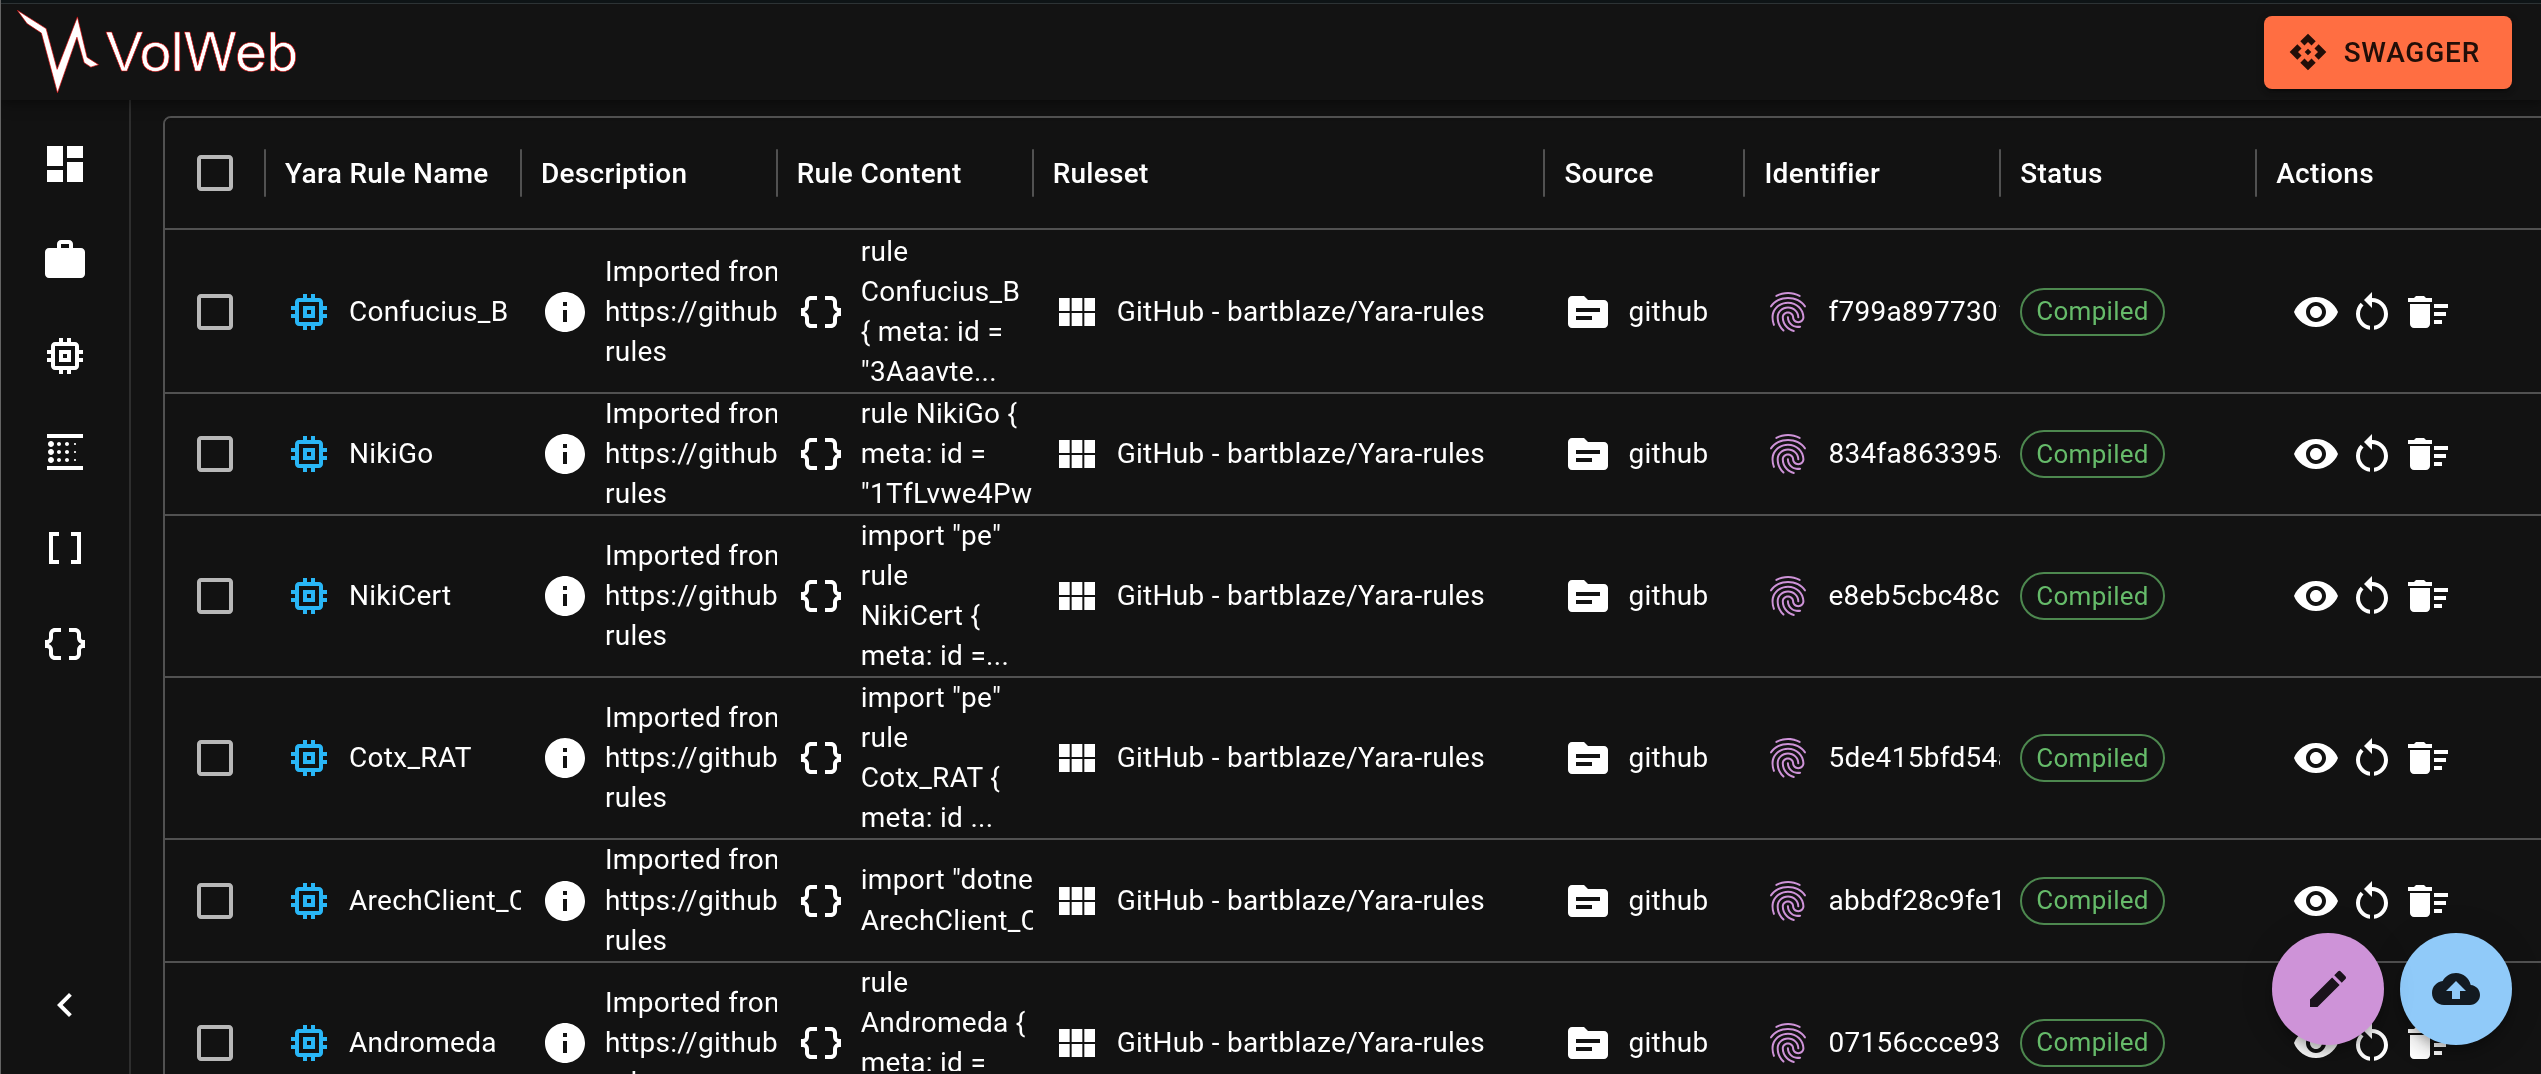
\includegraphics[width=1\linewidth]{images/volweb-esteso/volweb-rulelist.png}
\end{figure}

\subsubsection{Import e Creazione di Regole}

Il sistema di acquisizione delle regole supporta tre modalità principali: upload da file system, import da repository GitHub, e creazione manuale tramite editor integrato.

L'upload da file system implementa un'interfaccia che accetta la selezione di singoli file .yar. Il dialog consente la selezione della modalità di import (regola standalone, ruleset esistente, nuovo ruleset). Durante l'upload, una progress bar mostra l'avanzamento per file, con possibilità di cancellare upload in corso.

L'integrazione GitHub permette import diretto da repository pubbliche, eliminando il download manuale. Il sistema mantiene una lista curata di repository popolari (Yara-Rules, reversinglabs-yara, Neo23x0/signature-base) con accesso one-click. Per repository custom, l'utente può inserire l'URL e il sistema enumera automaticamente tutti i file .yar disponibili. Il sistema mantiene il riferimento alla fonte originale per facilitare aggiornamenti futuri.

L'editor integrato per creazione di regole custom fornisce un ambiente di sviluppo completo. Il componente, basato su Monaco Editor (lo stesso engine di VS Code), offre syntax highlighting specifico per YARA con colorazione differenziata per keywords, strings, e commenti. L'auto-completion suggerisce keywords YARA, nomi di variabili definite, e funzioni built-in mentre si digita. La validazione real-time sottolinea errori sintattici con squiggly lines rosse e mostra tooltip con descrizioni degli errori on hover.

\begin{figure}[H]
\centering
\begin{minipage}{0.45\textwidth}
\centering
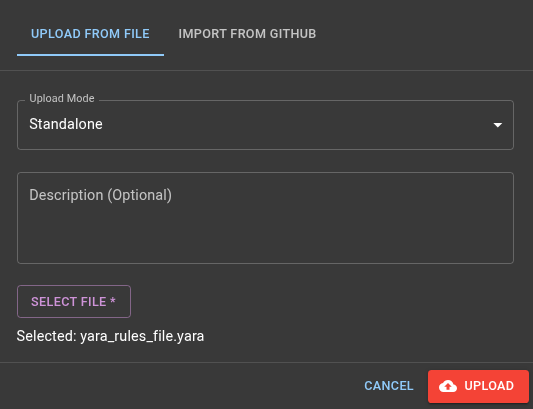
\includegraphics[width=\textwidth,height=6cm]{images/volweb-esteso/volweb-upload-dialog.png}
\end{minipage}
\hspace{0.05\textwidth}
\begin{minipage}{0.45\textwidth}
\centering
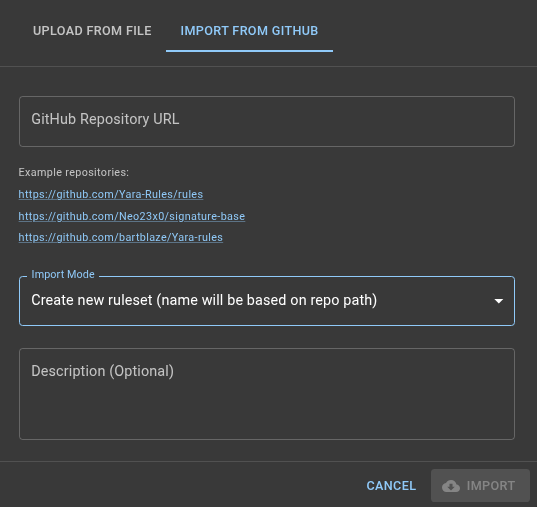
\includegraphics[width=\textwidth,height=6cm]{images/volweb-esteso/volweb-import-dialog.png}
\end{minipage}
\end{figure}

La gestione degli errori durante l'import è stata progettata per essere informativa senza essere overwhelming. Errori di validazione sono raggruppati per tipo e presentati in un formato scannable. Per ogni errore, il sistema mostra la linea esatta dove si verifica il problema, una descrizione human-readable dell'errore, e suggerimenti per la correzione quando possibili. Gli errori non bloccano l'import di altre regole valide, permettendo import parziali con report dettagliato di cosa è stato importato e cosa è fallito.

\subsubsection{Gestione dei RuleSets}

L'implementazione della dashboard dedicata ai ruleset é la stessa della dashboard delle regole, utilizzando Material-UI DataGrid con virtualizzazione delle righe per gestire efficientemente centinaia di ruleset senza degradazione delle performance.

Ogni riga mostra informazioni essenziali ottimizzate per scansione visiva rapida: il nome del ruleset, la sua descrizione, lo stato di compilazione e le azioni rapide disponibili.

Le azioni rapide disponibili per ogni ruleset sono: la visualizzazione dettagliata che reinvia alla vista espansa del ruleset con lista delle regole contenute e stato di ciascuna; la compilazione manuale che permette di ricompilare il ruleset in qualsiasi momento; l'eliminazione, che richiede conferma tramite dialog per prevenire cancellazioni accidentali.

\begin{figure}[H]
\centering
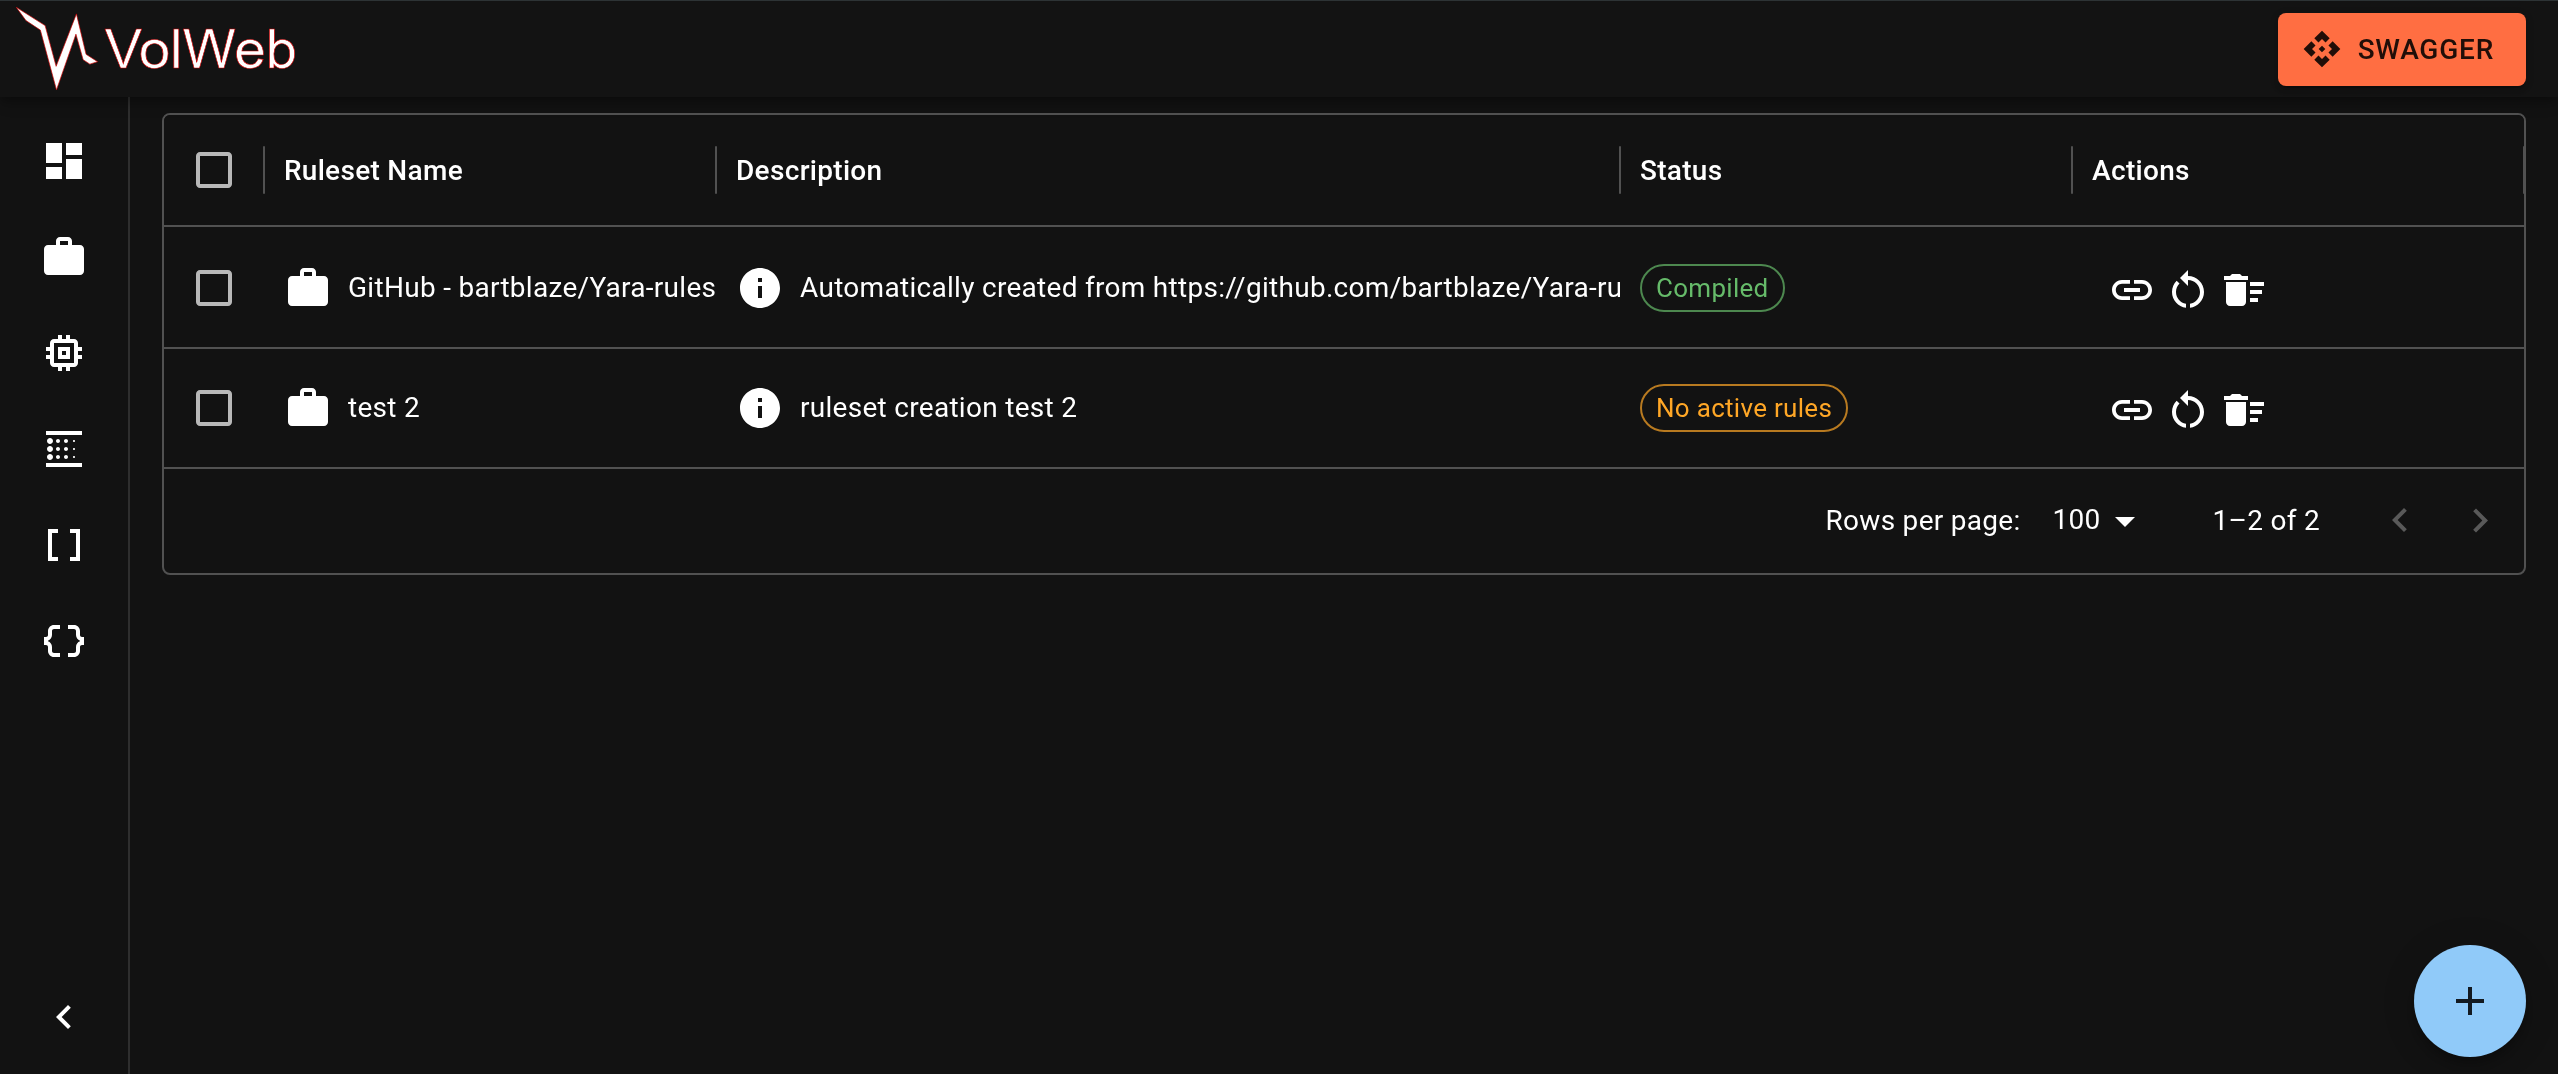
\includegraphics[width=1\linewidth]{images/volweb-esteso/volweb-rulesetlist.png}
\end{figure}

\subsubsection{Configurazione ed Esecuzione delle Scansioni}

L'interfaccia di scansione fornisce controllo sulla selezione delle regole utilizzando un'interfaccia a due pannelli con rulesets sulla sinistra e regole individuali sulla destra. Gli utenti possono selezionare interi rulesets, che automaticamente selezionano tutte le regole attive al loro interno, oppure selezionare regole individuali, o entrambe le modalità. É possibile, infine, selezionare tutti i rulesets e/o tutte le regole attive tramite checkbox dedicate.

Una volta selezionate le regole, l'utente può avviare la scansione, che viene eseguita in background tramite Celery. Al termine della scansione, l'utente viene notificato via WebSocket e può visualizzare i risultati dettagliati.

Alternativamente all'esecuzione di un nuovo scan, l'utente può visualizzare i risultati dell'ultimo scan eseguito sul dump selezionato, se disponibile. Questa funzionalità permette di rivedere rapidamente i risultati senza dover rieseguire la scansione.

\begin{figure}[H]
\centering
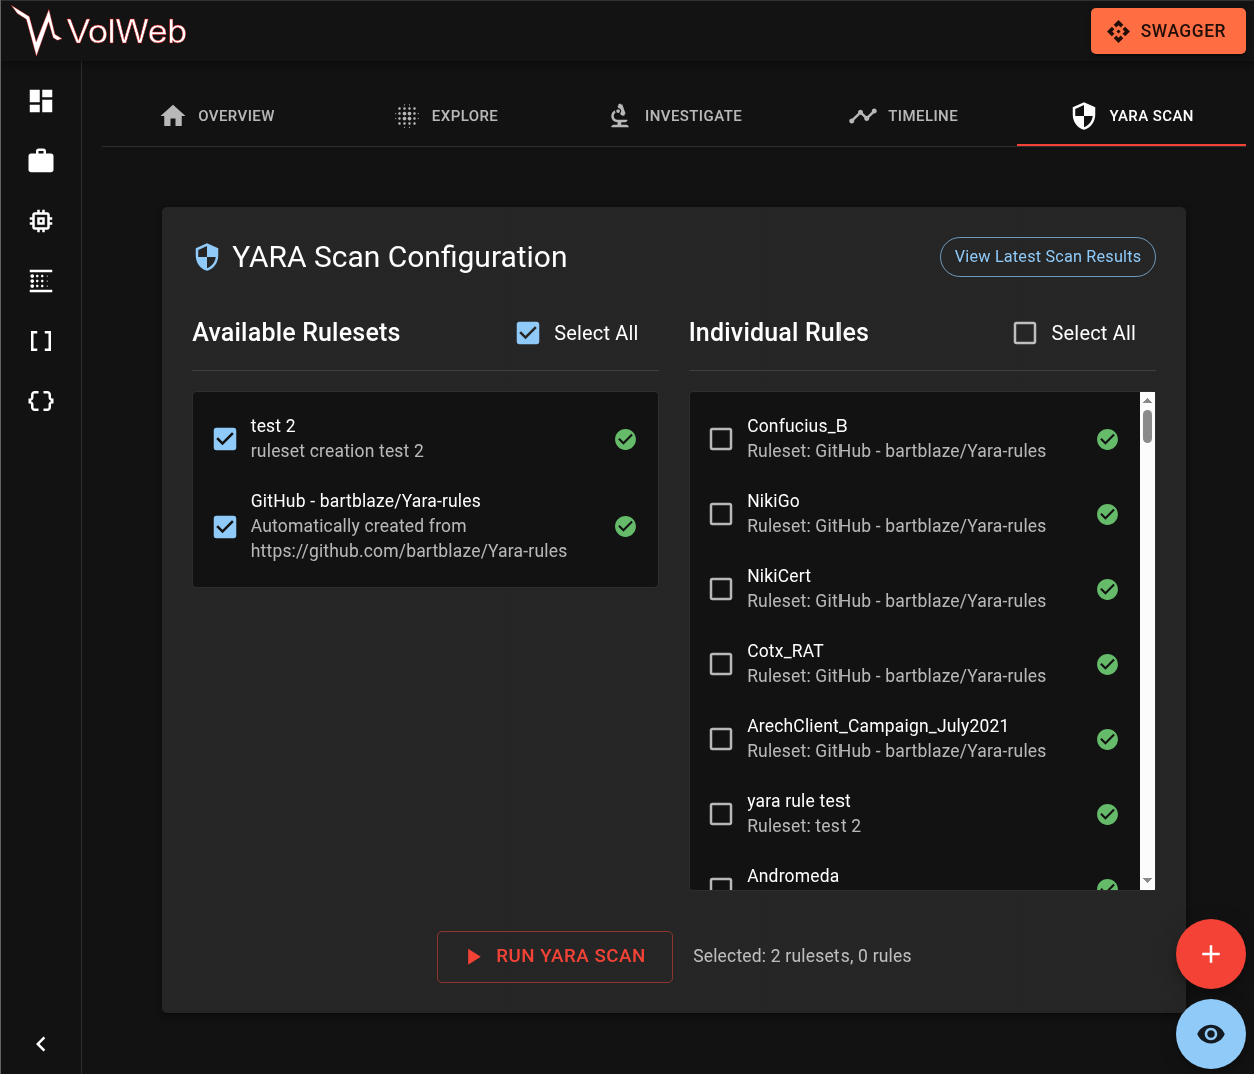
\includegraphics[width=1\linewidth]{images/volweb-esteso/volweb-scanview.png}
\end{figure}

\subsubsection{Visualizzazione e Analisi dei Risultati}

La presentazione dei risultati delle scansioni YARA é organizzata in una vista tabellare con funzionalità di filtering e sorting. 

La tabella, per ogni match, mostra il nome della regola che ha generato il match, il valore che ha causato il match, l'offset esatto nel dump e il componente della regola che é stato attivato.

É possibile eliminare i risultati dello scan corrente, che rimuove tutti i match associati al dump dal database, oppure eseguire un nuovo scan salvando i risultati appena visualizzati.

\begin{figure}[H]
\centering
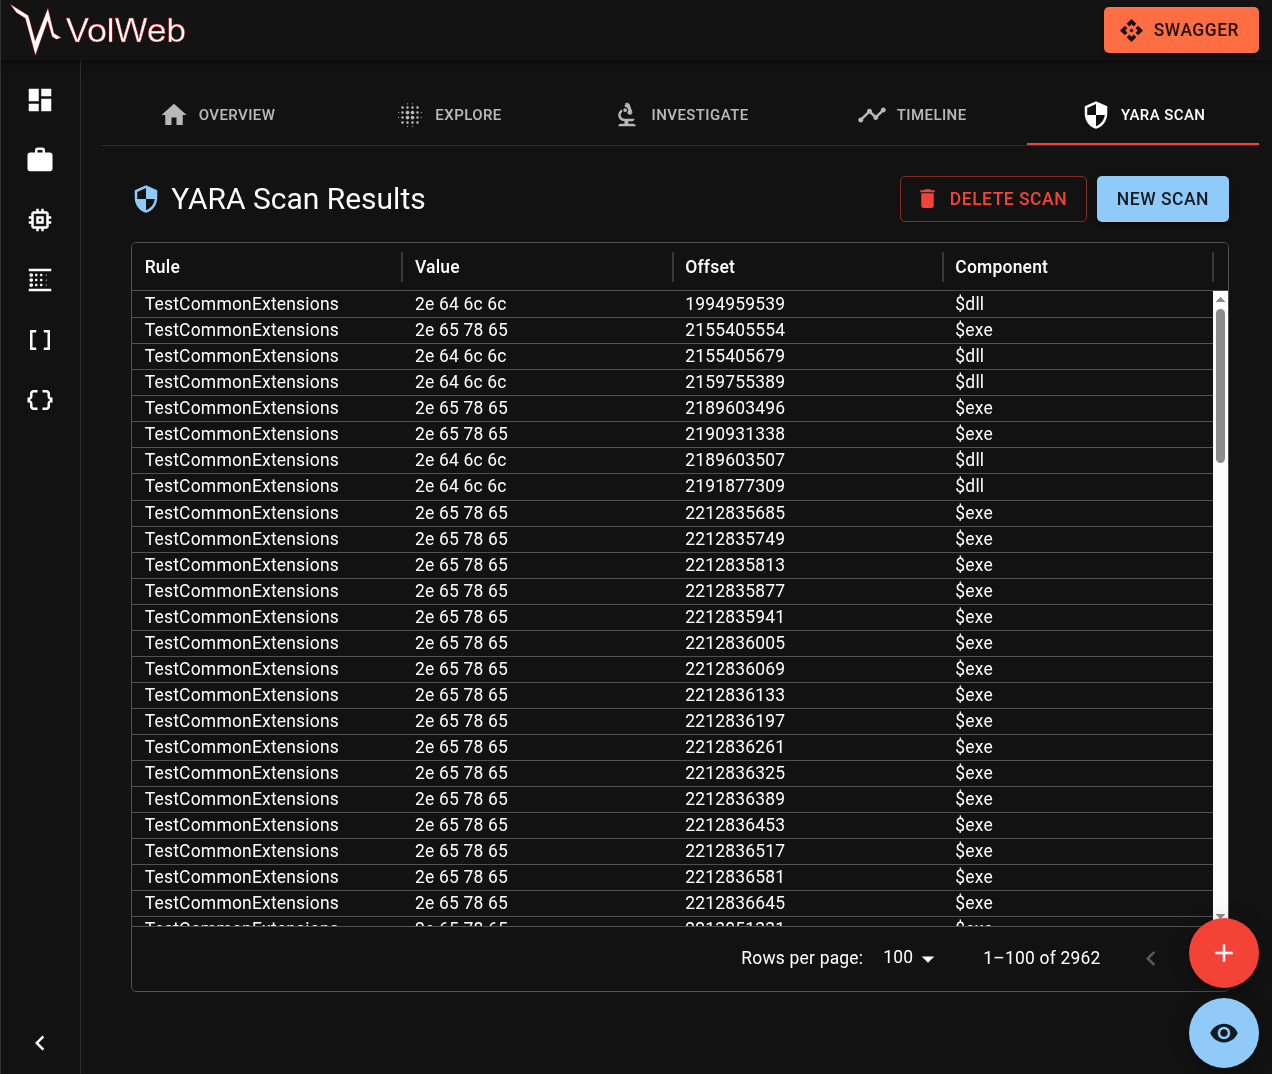
\includegraphics[width=1\linewidth]{images/volweb-esteso/volweb-scanresult.png}
\caption{Visualizzazione stratificata dei risultati YARA con drill-down progressivo dal summary al dettaglio forense}
\end{figure}

\section{Semplificazioni Architetturali}

Parallelamente all'integrazione YARA, sono state implementate semplificazioni architetturali significative basate sull'esperienza operativa di Locked Shields 2025.

\subsection{Rimozione del Sistema di Autenticazione}

L'eliminazione del layer di autenticazione rappresenta una decisione progettuale apparentemente controintuitiva che tuttavia riflette la realtà operativa degli ambienti forensi isolati. Durante Locked Shields 2025, ogni blue team operava in un ambiente di rete completamente segregato dove il controllo degli accessi era demandato all'infrastruttura di rete piuttosto che all'applicazione.

L'analisi dell'utilizzo durante l'esercitazione ha rivelato pattern interessanti. I team tipicamente deployavano VolWeb su una VM isolata accessibile solo dalla rete del team. L'accesso alla rete era già protetto da VPN con autenticazione multi-fattore. All'interno del team, tutti i membri necessitavano dello stesso livello di accesso. Il tempo speso per gestire account utente e password reset durante l'esercitazione rappresentava overhead non produttivo.

Ancora più critico, il sistema di autenticazione rappresentava un vettore di attacco sfruttabile. Durante le simulazioni, i red team targetizzavano specificatamente i sistemi di autenticazione delle applicazioni web.

L'architettura risultante assume che VolWeb venga deployato in ambienti trusted dove la sicurezza perimetrale è già garantita. Questo modello si allinea con il principio di defense in depth, dove la sicurezza non dipende da un singolo controllo ma da layer multipli. Per deployment che richiedono autenticazione, il sistema può essere protetto attraverso reverse proxy (nginx, Apache) con autenticazione integrata, VPN con controlli di accesso basati su certificati, o network segmentation con firewall rules.

\subsection{Eliminazione del Supporto Cloud Storage}

La rimozione del supporto per storage cloud deriva da considerazioni pratiche e di sicurezza emerse durante operazioni reali. L'analisi post-Locked Shields ha rivelato che zero team su 40 hanno utilizzato il cloud storage durante l'esercitazione, nonostante fosse disponibile e configurato.

Le ragioni per il non-utilizzo erano molteplici. Dal punto di vista della sicurezza, i dump di memoria contengono inevitabilmente dati estremamente sensibili. L'upload automatico di tali dati su infrastrutture cloud viola multiple normative di compliance, GDPR per dati personali EU, HIPAA per informazioni sanitarie, PCI-DSS per dati di pagamento, e classificazioni governative per informazioni sensibili.

Dal punto di vista operativo, la dipendenza da servizi cloud introduceva failure points inaccettabili. Durante Locked Shields, i servizi cloud simulati erano tra i primi target degli attacchi red team. In uno scenario reale di incident response, questi problemi sarebbero ancora più critici quando l'infrastruttura aziendale è sotto attacco.

Le considerazioni di performance hanno ulteriormente supportato la decisione. L'upload di dump da 20-64 GB su connessioni internet standard richiedeva ore. Il download per analisi introduceva latenza significativa. I costi di storage e bandwidth per dump multipli diventavano rapidamente proibitivi. La sincronizzazione tra storage locale e cloud aggiungeva complessità senza valore evidente.

L'implementazione della rimozione ha richiesto un refactoring significativo ma ha prodotto un'architettura più semplice e robusta. 

Le espansioni presentate in questo capitolo trasformano VolWeb da una piattaforma di visualizzazione a uno strumento completo per l'analisi forense avanzata. L'integrazione di YARA colma il gap più critico identificato durante Locked Shields 2025, fornendo capacità di pattern matching e threat hunting precedentemente assenti. Le semplificazioni architetturali garantiscono che la piattaforma rimanga accessibile e resiliente anche nei contesti operativi più impegnativi, rimuovendo complessità non necessaria e potenziali punti di failure.

L'implementazione dettagliata, comprensiva di tutto il codice sorgente, è disponibile nel repository GitHub del progetto, come documentato nell'Appendice A.

Il capitolo successivo discuterà i test di validazione eseguiti per garantire che le nuove funzionalità soddisfino i requisiti definiti, seguiti da una valutazione complessiva dell'impatto delle espansioni sulla piattaforma VolWeb.
\include{conclusioni} 
\bibliographystyle{unsrturl}  
\bibliography{bibliografia}
\include{ringraziamenti}
\end{document}
